\part{光线追踪}

\chapter{阴影}

在着色这一部分, 我们介绍了如何对各个物体计算对应像素的颜色. 然而, 我们的计算对于每个模型来说都是独立的, 并没有考虑光的遮挡关系. 因此我们在这里说明在光栅化的情况下, 如何计算阴影. 

\section{Shadow Mapping}
\textbf{Shadow Mapping}是一种图像空间的算法. 在计算阴影的时候我们不需要知道场景的几何信息. Shadow Mapping的方法只适用于在点光源下计算硬阴影.
硬阴影指的是一个点是否在阴影内是确定的, 它不是在阴影内就在阴影外; 只有点光源才可以产生这种情况. 软阴影指的是阴影是有过渡的, 一个点可以接收到部分光线; 当不忽略光源大小的时候, 就会产生这种情况.
可以接收到部分光线的区域一般称为半影. 

一个点是否在阴影中取决于光源和摄像机是不是都可以看到这个点. 如果都可以看到这个点, 那么说明这个点不在阴影里. 因此我们使用如下方式进行计算: 
\begin{enumerate}
	\item 从光源位置看向场景, 做出深度图; 
	\item 从摄像机位置看向场景, 对于每一个看到的点, 计算到光源的距离, 并且得到光源深度图上对应像素点的距离进行比较. 如果距离一样, 那么说明这个点不在阴影中, 反之, 这个点在阴影中. 
\end{enumerate}

这样的算法有两个问题: 
\begin{enumerate}
	\item 距离是一个浮点数, 不容易进行比较. 需要引入一定的宽容度. 这是数值精度的问题, 不能从本质解决问题; 
	\item 阴影的质量和光源深度图的分辨率有关. 如果光源深度图太小, 但是摄像机分辨率大就容易出现走样问题; 
	\item 这个方法只适合硬阴影, 不适合软阴影. 
\end{enumerate}

因此, 我们需要引入光线追踪的方法来解决光栅化Shadow Mapping中可能出现的问题. 

\begin{figure}[H]
	\centering
	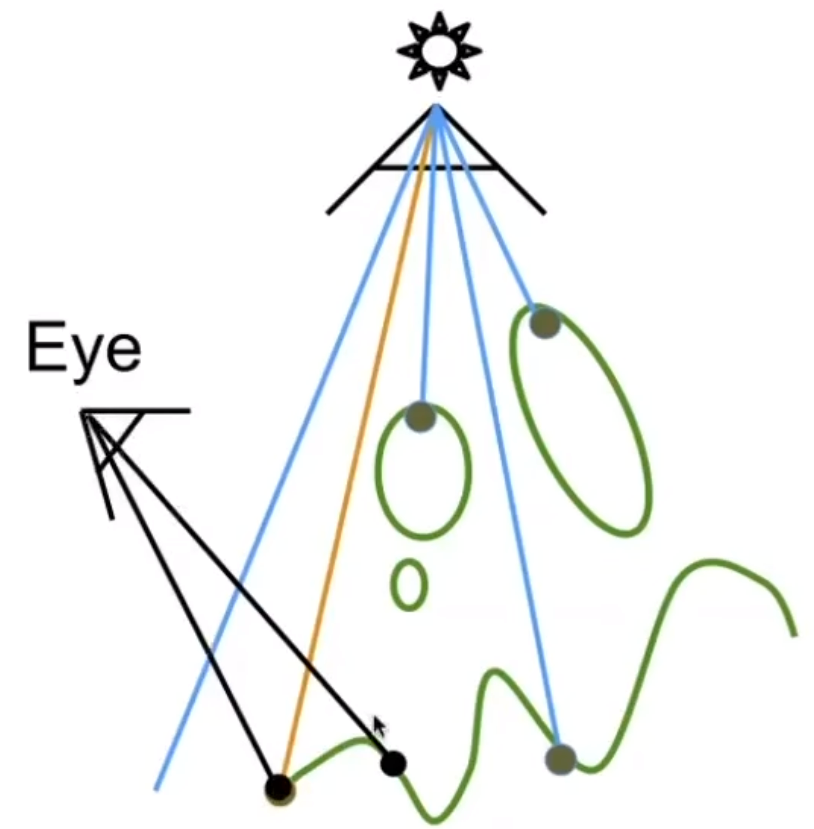
\includegraphics[scale=.5]{ShadowMapping_1.png}
	\caption{相机视角的深度与点光源视角的深度一致, 可见}
	\label{fig:ShadowMapping_1}
\end{figure}

\begin{figure}[H]
	\centering
	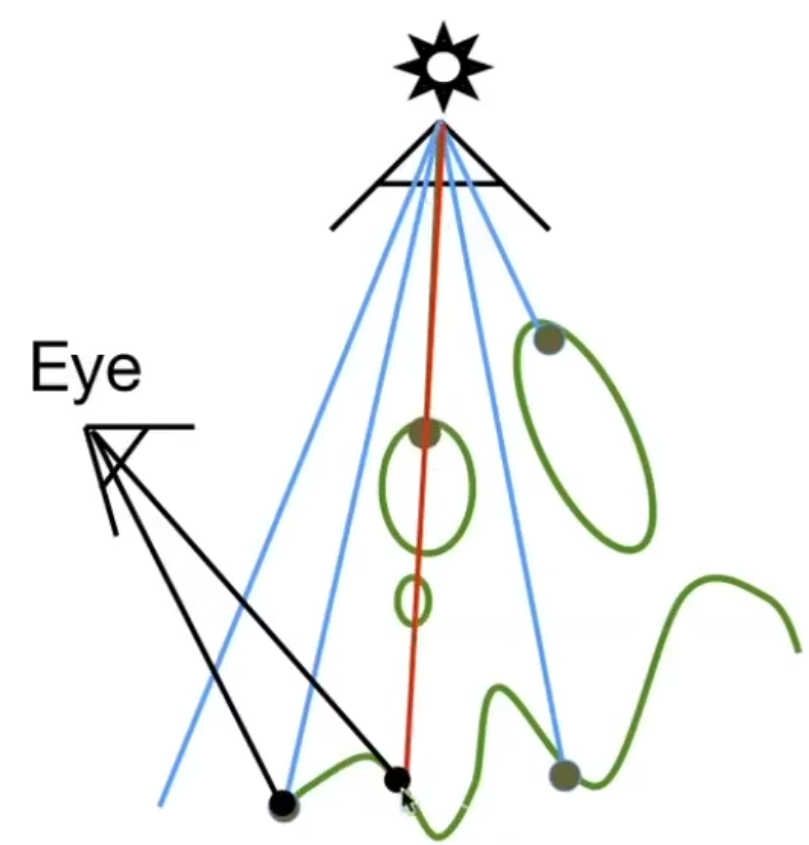
\includegraphics[scale=.5]{ShadowMapping_2.png}
	\caption{相机视角的深度与点光源视角的深度不一致, 不可见}
	\label{fig:ShadowMapping_2}
\end{figure}





\chapter{光线追踪}

\section{基础知识}

我们引入光线追踪, 主要是为了解决光栅化中没有解决的一些问题: 
\begin{enumerate}
	\item 全局的光照效果不好表示; 
	\item 软阴影效果的产生; 
	\item 光泽反射 (Glossy reflection, 一种类似于镜面反射的情况, 但是没有镜面光滑的表面产生的情况) 会让光线在场景中多次反射; 
	\item 间接光照, 在漫反射场景中, 有些光线在到达眼睛前反射不止一次. 
\end{enumerate}

光栅化是一种比较快速, 近似的一种渲染方式, 用于实时渲染; 光线追踪是比较准确但是比较慢的渲染方式, 用于离线渲染. 

\subsection{基本光线追踪方法}

\subsubsection{光线的定义}

我们假设光线有以下三个性质: 
\begin{enumerate}
	\item 光沿直线传播; 
	\item 光线和光线不会发生碰撞的交叉; 
	\item 光线从光源射入人眼中. 
\end{enumerate}
因此我们可以利用光的可逆性 (Reciprocity) 进行光线追踪. 光线追踪是指我们从摄像机沿着每一个像素点的连线射出光线, 追踪光线的路径. 

\subsubsection{光线追踪的假设}
我们认为眼睛是一个点, 光源均为点光源. 我们从眼睛沿着像素点画一条光线, 如果光线和物体有接触, 我们将交点和光源进行连线, 如果可以连接到光源, 那我们认为这一点被照亮, 可以计算着色. 

\subsection{Whitted-Style光线追踪}
从眼睛沿着像素连接一条光线, 我们认为光线在传播的过程中发生反射和折射现象. 假设反射是完美的镜面反射. 当我们将所有的反射 (折射) 点和光源连接起来. 如果这一点可以被光源照亮, 那么我们认为这一点的着色应当叠加在这个像素上. 对于光线我们认为存在能量的消逝, 不会一直反射. 

\begin{figure}[H]
	\centering
	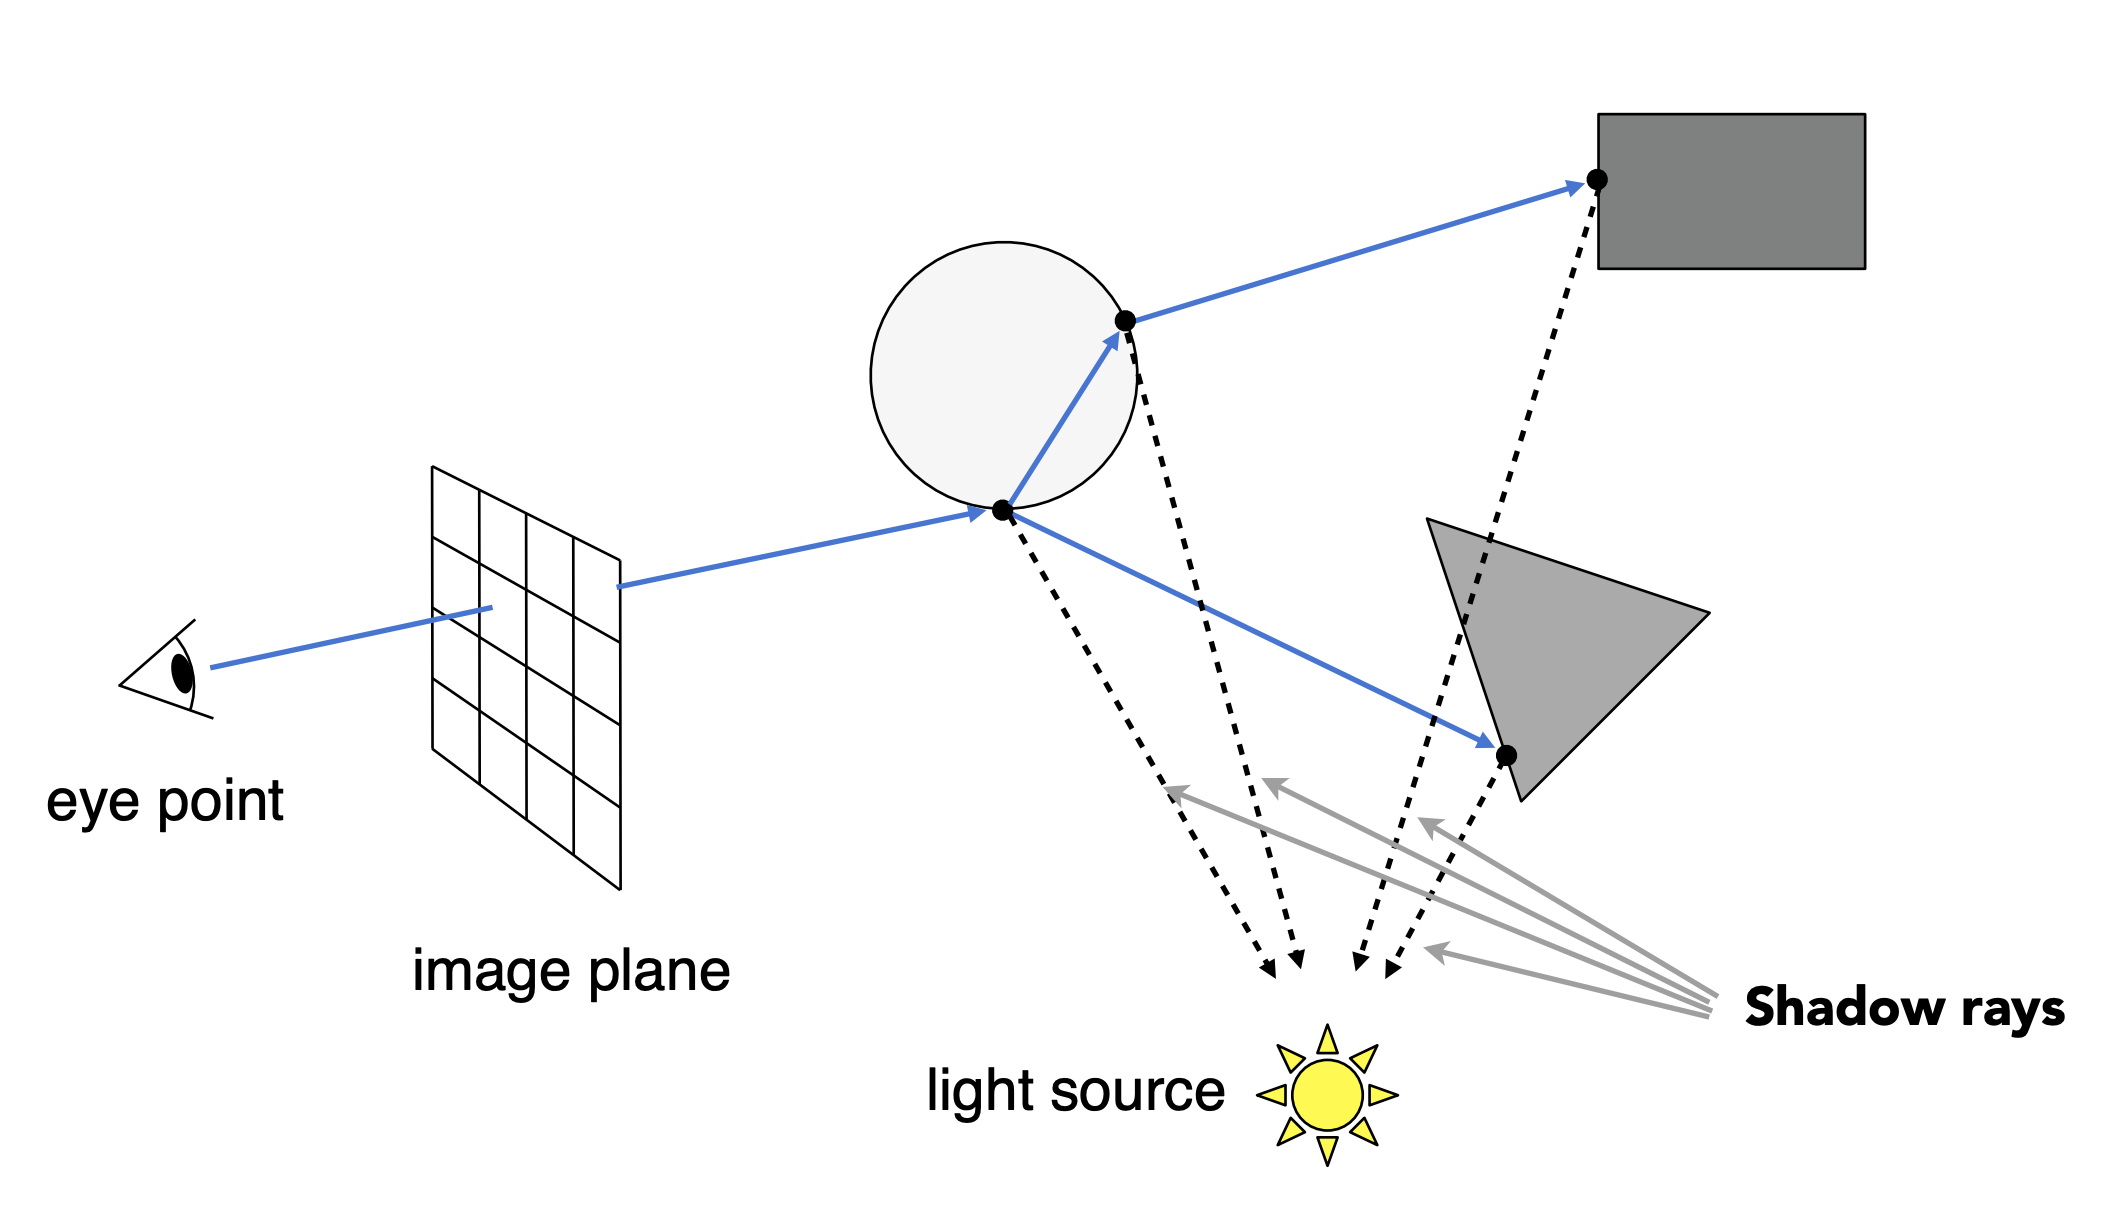
\includegraphics[scale=.25]{guangxianzhuizong.png}
	\caption{Whitted-Style光线追踪示意图}
	\label{fig:gxzz}
\end{figure}
眼睛和像素直接连接起来的光线称为primary ray, 发生反射和折射后形成的光线称为secondary ray, 反射点和光源的连线称为shadow ray. 

\subsection{光线-表面交点}
对于光线追踪而言, 最重要的就是求出光线和物体的交点. 首先我们对光线进行定义. 我们假设光线的起点为$o$, 光线的方向是单位向量$d$, 那么光线就可以定义为$o+td$. 

\subsubsection{光线和球面的交点}

我们首先计算光线和球面的交点作为引入. 光线我们可以表示为: 
\begin{equation}
	r(t)=o+td, 0\le t \le \infty
\end{equation}

对于球面, 我们可以表示为: 
\begin{equation}
	(p-c)^2-R^2=0
\end{equation}其中, $c$是球心, $p$是任意一点. 如果$p$是光线和球面的交点, 那么这个点可以同时满足上面两个函数. 因此, 我们将光线公式代入到球面公式上就可以得到它们的交点: 
\begin{equation}
	(o+td-c)^2-R^2=0
\end{equation}
这是一个二元一次方程组, 使用求根公式就可以得到结果. 我们讨论求根公式中$\triangle$值. 如果$\triangle < 0$, 那么光线和球体没有交点; 如果$\triangle = 0$, 光线和球体相切; 如果$\triangle > 0$, 那么光线穿过球体, 有两个交点. 

\subsubsection{光线和隐式函数面的交点}

光线我们可以表示为: 
\begin{equation}
	r(t)=o+td, 0\le t \le \infty
\end{equation}

对于任意一个隐式函数面, 我们定义为: 
\begin{equation}
	f(p)=0
\end{equation}

我们可以直接把光线公式代入隐式函数中求出结果: 
\begin{equation}
	f(o+td)=0
\end{equation}

\subsubsection{光线和显式三角形面的交点}
我们可以通过求交点的方式判断一个点是否在封闭曲面的内部还是外部. 任何一个点发出一条光线, 如果交点个数为奇数, 那么这个点一定在封闭曲面内部; 如果有偶数个点, 那么这个点一定在封闭曲面的外部. 

我们求一条光线和显式三角形面的交点可以分为两步: 
\begin{enumerate}
	\item 求出光线和三角形面所在平面的交点; 
	\item 判断这个点是否在三角形内 (之前的课程中已经介绍了判断的方法) . 
\end{enumerate}

我们使用法线$N$和平面上的任意一个点$p‘$来定义一个平面: 
\begin{equation}
	(p-p')\cdot N = 0
\end{equation}
其中$p'$是平面上任意一点, 满足条件的$p$都在这个平面上. 我们令$p=o+td$就可以求出光线和这个平面的交点, 
\begin{equation}
	(p-p')\cdot N = (o+td-p')\cdot N = 0
\end{equation}
可以求出: 
\begin{equation}
	t = \frac{(p'-o)\cdot N}{d\cdot N}, 0\le t \le \infty
\end{equation}

我们可以通过另一种算法直接求出一条光线和一个显式三角形面是否有交点. 任何一个显式的三角形内部的一个点都可以写成三个顶点的线性组合. 因此我们可以得到: 
\begin{equation}
	o+td=(1-b_1-b_2)P_0+b_1P_1+b_2P_2
\end{equation}使用克莱姆法则可以得到: 
\begin{equation}
	\begin{bmatrix}
		t\\ 
		b_1\\ 
		b_2
	\end{bmatrix}=\frac{1}{S_1\cdot E_1}\begin{bmatrix}
		S_2\cdot E_2\\ 
		S_1\cdot E\\ 
		S_2\cdot D
	\end{bmatrix}
\end{equation}其中, $E_1=P_1-P_0,E_2=P_2-P_0,S=O-P_0,S_1=D\times E_2, S_2=S\times E_1$.最后我们只需要判断这个解是否合理即可, 只要求解出的三个量都是非负的, 那么光线和显式三角形面有一个交点. 

\section{光线追踪加速}
传统的计算方法所需要的计算消耗量非常大, 因此我们需要通过一些方式加速计算. 
\subsection{包围体积}
\textbf{包围体积 (Bounding Volume) }使用一个简单的立方体包围复杂的模型. 如果光线连包围盒都碰不到, 那么光线一定不能碰到里面的物体. 
我们常用的包围盒是\textbf{轴对其包围盒 (Axis-Aligned Bounding Box,  AABB) }, 包围盒的长宽高和坐标轴都是平行的. 我们认为, 包围体积是三组成对平面的交集. 为了计算光线和包围盒的相交情况, 我们在二维情况下进行简化计算: 
\begin{figure}[H]
	\centering
	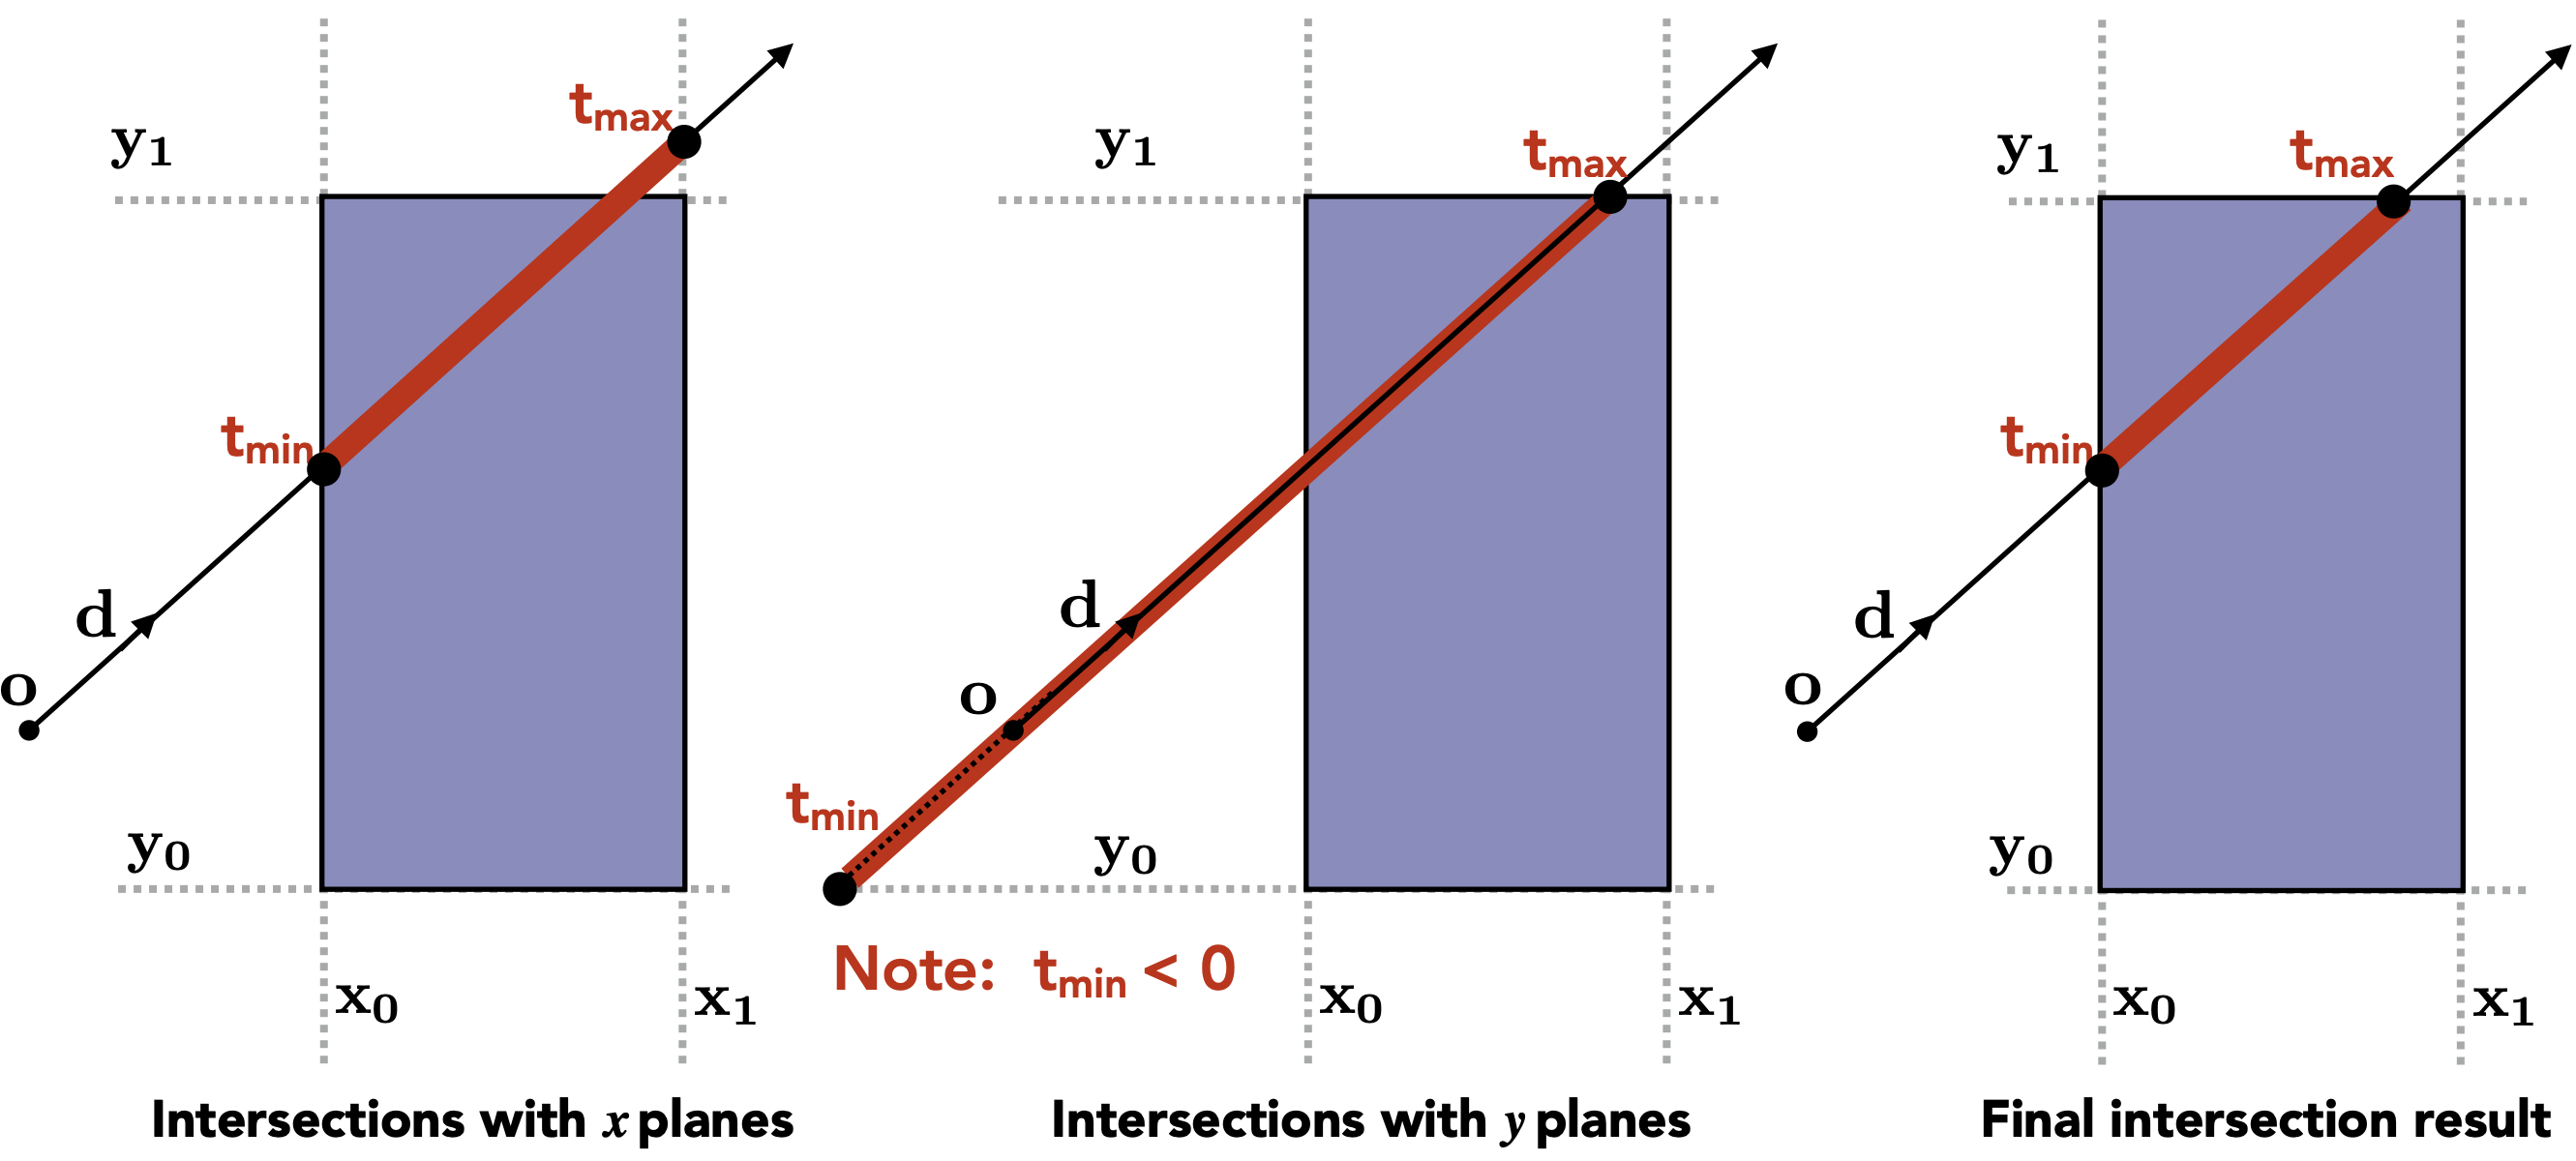
\includegraphics[scale=.25]{baoweitiji.png}
	\caption{包围体积中交点的计算}
	\label{fig:bwtj}
\end{figure}

我们求出光线在x平面上的两个交点以及y平面上的两个交点, 那么最终光线在包围盒内部的部分是这些交点区间的交集. 我们可以认为: 
\begin{itemize}
	\item 光线进入到三个面中, 才可以进入到包围盒; 
	\item 光线离开任意一个面, 就会离开包围盒. 
\end{itemize}
我们对三对面分别求出进入时间$t_{min}$和离开时间$t_{max}$, 那么最终对于包围盒来说进入时间$t_{enter}$是所有进入时间的最大值, 离开时间$t_{exit}$是所有离开时间的最小值. 如果进入时间小于离开时间, 那么我们认为光线和盒子有交点. 

对于时间出现负值的情况, 我们进行以下讨论: 
\begin{itemize}
	\item 如果离开时间$t_{exit}<0$, 那么盒子在光线的背后, 不会产生交点; 
	\item 如果进入时间$t_{enter} < 0$, 那么光线的起点在盒子的里面. 
\end{itemize}

光线和盒子有交点, 当且仅当 (iff) $t_{enter}<t_{exit}, t_{exit}\geq 0$.
我们可以利用三角形相似性求出对应的$t$值. 
\begin{figure}[H]
	\centering
	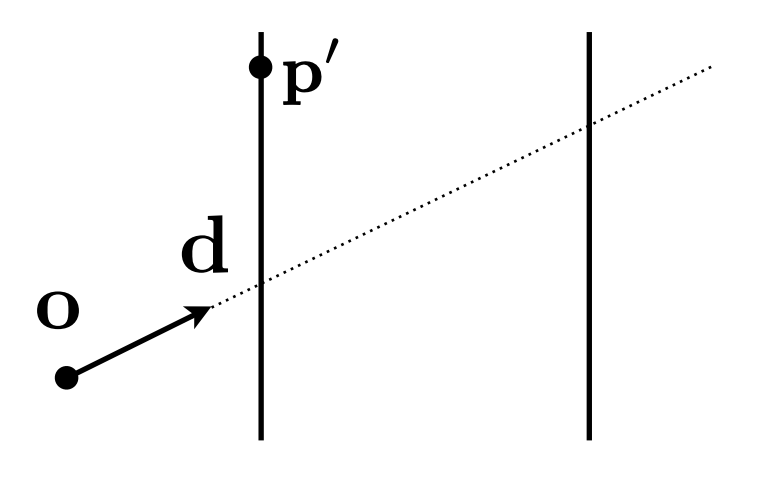
\includegraphics[scale=.25]{AABB.png}
	\caption{AABB中$t$值的计算}
	\label{fig:aabb}
\end{figure}
$t$值可以表示为: 
\begin{equation}
	t=\frac{p'_x-o_x}{d_x}
\end{equation}

\subsection{空间划分}
为了可以加速光线和物体求交点, 我们可以使用网格将原本比较大的包围盒进行划分. 我们进行网格划分分为以下几个步骤: 
\begin{enumerate}
	\item 找到场景中的包围盒; 
	\item 将包围盒划分成一个一个小格子; 
	\item 存储哪些小格子中包含物体 (我们认为物体都是非实心的面, 只记录包含面的小格子, 物体内部不包含面的小格子不计入) ; 
	\item 判断光线是否和格子相交, 如果光线和某个格子相交并且这个格子中包含物体, 那么我们需要与格子中的物体求光线的交点 (这里有两个假设: 1.判断光线和格子是否相交是很快的; 2.我们可以使用计算机图形学中画直线的方法来判断哪些格子是会相交的. ) . 
\end{enumerate}
\begin{figure}[H]
	\centering
	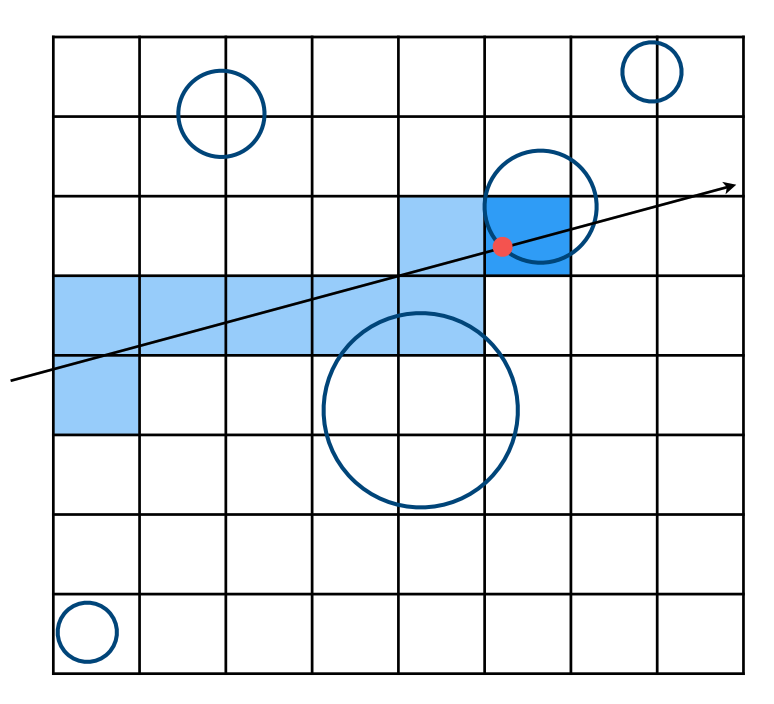
\includegraphics[scale=.15]{wanggehuafen.png}
	\caption{网格划分}
	\label{fig:wghf}
\end{figure}
一般来说, 格子的划分不可以太稀疏也不可以太稠密, 需要对格子的量进行控制. 这种划分方式对于物体分布均匀的场景比较合适. 对于物体分布稀疏的场景需要多次和格子进行相交判断, 这种方法相对不合适. 

我们会使用其他空间划分方法, 包括八叉树 (Oct-Tree) , KD树 (KD-Tree) 以及BSP树 (BSP-Tree) . 
\begin{figure}[H]
	\centering
	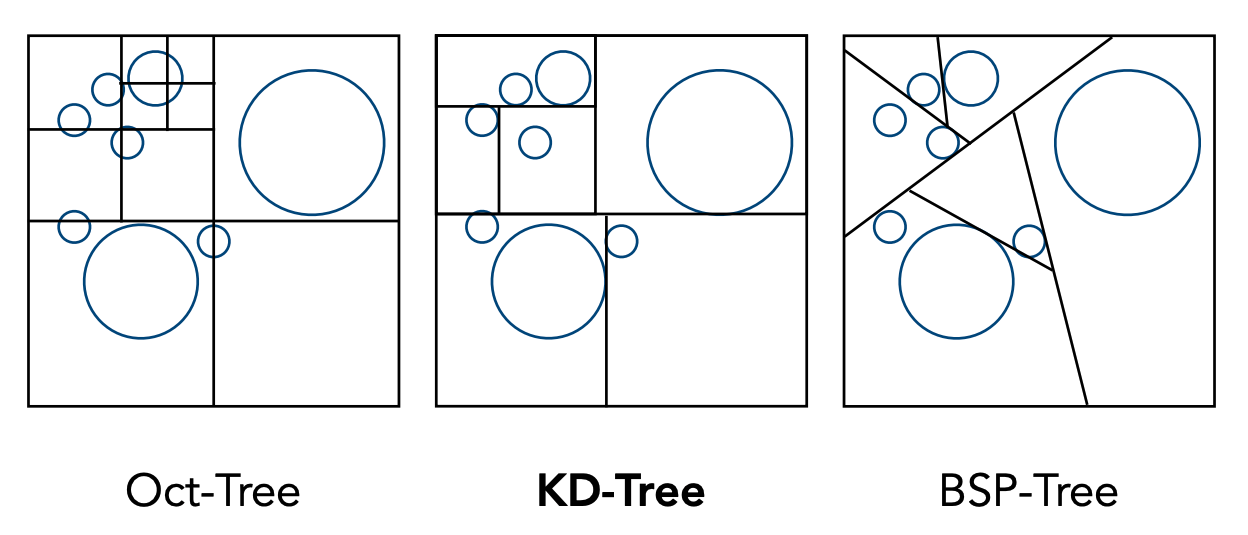
\includegraphics[scale=.15]{kongjianhuafen.png}
	\caption{空间划分}
	\label{fig:kjhf}
\end{figure}
\begin{itemize}
	\item \textbf{八叉树 (Oct-Tree) }, 将一个包围盒切成八块 (图中是二维情况, 只有4块) . 对于每一个小格子我们会继续进行划分直到小格子中没有物体或者物体的数量比较少; 
	\item \textbf{KD树 (KD-Tree) }, 每一次都进行一次水平划分或者竖直划分, 将包围盒分成两部分. 可以形成一个二叉树的存储结构. 水平划分和竖直划分交替进行, 保证划分的空间是均匀的; 
	\item \textbf{BSP树 (BSP-Tree) }, 每一次选择一个方向进行一次划分, 并不是沿着轴平行方向划分. 
\end{itemize}
三种划分方法, KD树更常用并且使用起来比较方便, 可以用二叉树来存储. 在每一个二叉树节点中, 我们都要储存以下信息: 
\begin{itemize}
	\item 如果是非叶子结点, 需要存储划分轴, 划分的位置以及孩子节点的指针; 
	\item 如果是叶子结点, 需要存储格子中包含的物体. 
\end{itemize}

实际划分出的盒子均在叶子结点上. 

\begin{figure}[H]
	\centering
	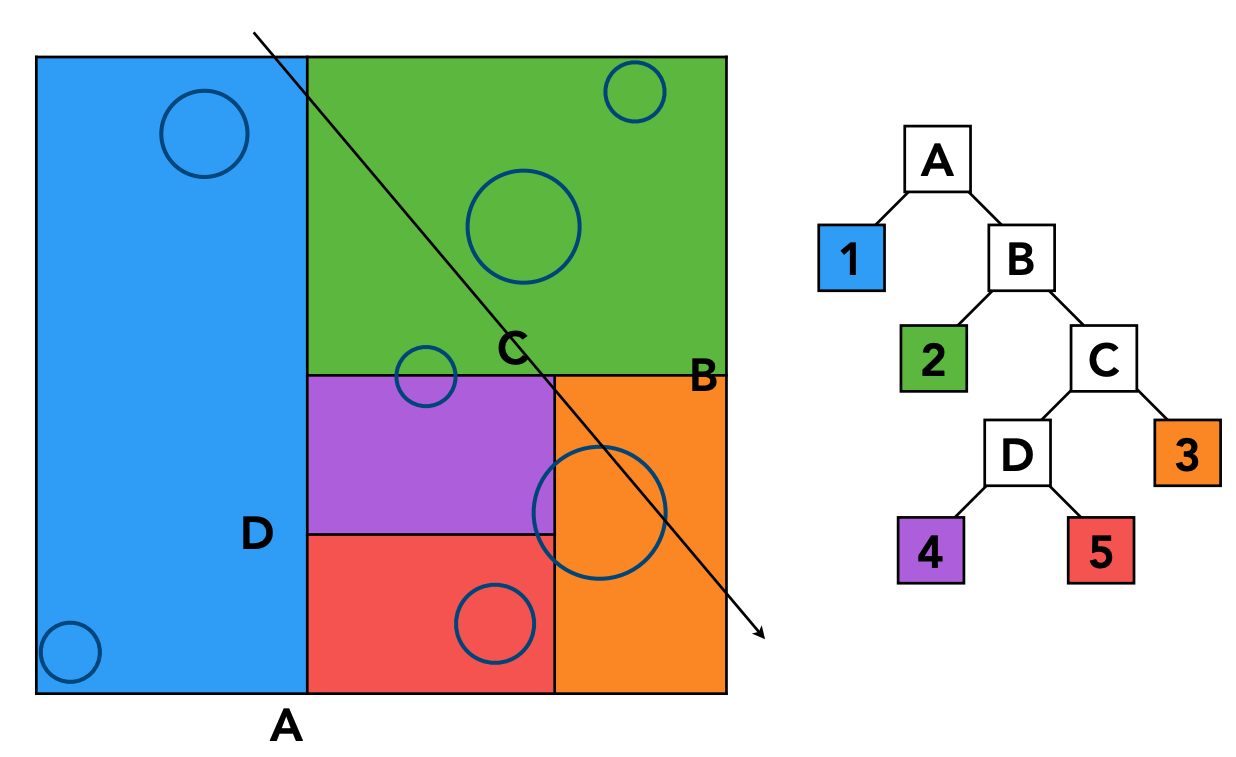
\includegraphics[scale=.15]{kongjianhuafenjisuan.png}
	\caption{空间划分后计算光线和物体的交点}
	\label{fig:kjhfjs}
\end{figure}
我们通过类似于二分查找的方式计算交点: 
\begin{itemize}
	\item 如果光线和一个节点有交点, 那么它和它的子节点也有交点; 
	\item 如果光线和叶子结点有交点, 那么它需要和格子内的所有物体求交点. 
\end{itemize}
这种方法存在两个问题, 首先, 格子和一个三角形面是否相交的判断比较复杂. 第二, 一个物体可能会在多个不同的格子中, 需要多次存储. 因此我们会使用更常用的物体划分的方式. 

\subsection{物体划分}
\textbf{物体划分 (Bounding Volume Hierarchy, BVH) }的主要思想是对物体进行进行划分, 并重新计算包围盒. BVH中, 每一个物体只属于一个包围盒. BVH的划分主要分为三步: 
\begin{enumerate}
	\item 划分包围盒; 
	\item 递归的将包围盒划分为两部分; 
	\item 当叶子结点的三角形面数量足够少的时候, 停止划分. 
\end{enumerate}
当我们进行划分的时候, 也有不同的划分技巧: 
\begin{itemize}
	\item 沿着最长的轴划分为两半 (让长轴变短, 分割更加均匀) ; 
	\item 取中间的物体进行划分, 可以保证两边三角形数量差不多 (找到第k个物体的算法可以在$o(n)$的时间内解决, 被称作快速选择算法) ; 
	\item 当包围盒中的物体数量小于一定数量的时候停止划分. 
\end{itemize}
使用伪代码可以写成如下形式: 
\begin{lstlisting}[
	caption={BVH伪代码},
	language=c]
	Intersect(Ray ray, BVH node) {
		if (ray misses node.bbox) return;
		
		if (node is a leaf node)
			test intersection with all objs;
			return closest intersection;
		
		hit1 = Intersect(ray, node.child1);
		hit2 = Intersect(ray, node.child2);
		return the closer of hit1, hit2;
	}
\end{lstlisting}
这是一个递归算法. 

\chapter{辐射度量学}
不论是光栅化还是光线追踪, 都是对我们现实光照的近似表示. 因此我们提出辐射度量学通过精准的物理定义模拟光照环境, 使用更真实的方式进行光线追踪. 辐射度量学描述了Radiant flux, intensity, irraddiance以及radiance. 

\section{Radiant Energy and Flux}
\textbf{Radiant Energy} 指的是电磁辐射的能量. 用符号$\mathbf{Q}$表示, 单位是焦耳$\mathbf{J}$.

\textbf{Radiant Flux (Power) } 指的是单位时间的能量. $\Phi=\frac{dQ}{dt}$, 单位是瓦特$\mathbf{W}$,也可以用单位$\mathbf{lm}$叫做流明 (lumen) . 是单位时间通过一个平面光照的量. 

\section{Radiant Intensity}
\textbf{Radiant Intensity}指的是光源在单位立体角上的能量. 数学定义为: 
\begin{equation}
	I(\omega)=\frac{d\Phi}{d\omega}
\end{equation} 单位为$\mathbf{W}/\mathbf{sr}$或者坎德拉$\mathbf{candela}=\mathbf{cd}=\frac{\mathbf{lm}}{\mathbf{sr}}$.

\subsection{单位立体角}
在二维平面上, 我们使用弧度制定义角度, 定义为角度对应圆上的弧长除以半径: 
\begin{equation}
	\theta = \frac{l}{r}
\end{equation} 单位是$\mathbf{rad}$.整圆对应的角度为$2\pi\ \mathbf{rad}$.

我们定义立体角为角度在球上对应的面积除以半径的平方: 
\begin{equation}
	\omega=\frac{A}{r^2}
\end{equation} 单位是$\mathbf{sr}$, 整球对应的立体角为$4\pi\ \mathbf{sr}$.

接下来我们推出\textbf{单位立体角 (Differential Solid Angles) }的公式: 
\begin{figure}[H]
	\centering
	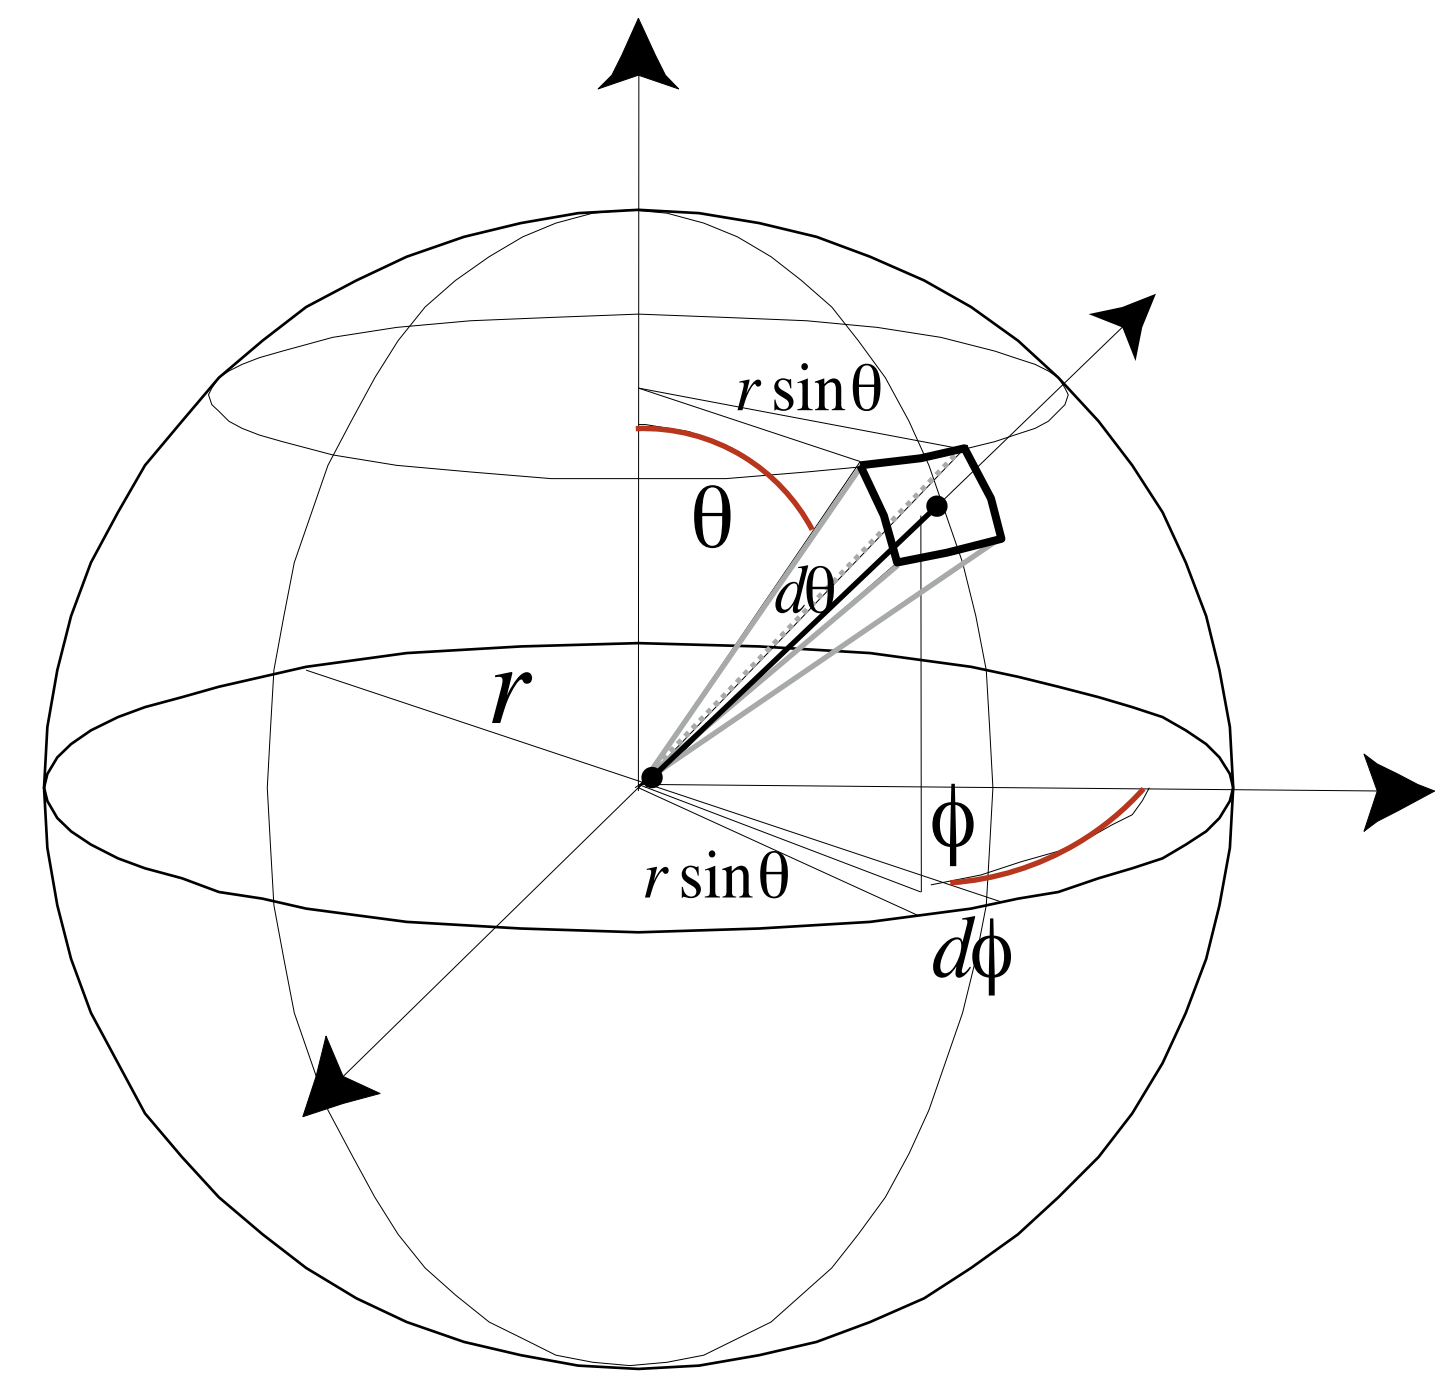
\includegraphics[scale=.25]{danweilitijiao.png}
	\caption{单位立体角推理}
	\label{fig:dwltj}
\end{figure}

\begin{equation}
\begin{split}
	dA=(rd\theta)(r\sin \theta d \phi)=r^2\sin\theta d\theta d\phi \\
	d\omega=\frac{dA}{r^2}=\sin\theta d\theta d\phi
\end{split}
\end{equation}

我们使用积分进行验证, 对整个球面的单位立体角进行积分: 
\begin{equation}
	\begin{split}
		\Omega=\int_{S^2}d\omega=\int_{0}^{2\pi}\int_{0}^{\pi}\sin\theta d\theta d\phi = 4\pi
	\end{split}
\end{equation}

因此, 对于一个均匀发光的光源, $I=\frac{\Phi}{4\pi}$. 

\section{Irradiance}

\textbf{Irradiance}指的是单位面积上所接收到的能量. 定义为: 
\begin{equation}
	E(x)=\frac{d\Phi(x)}{dA\cos\theta}
\end{equation} 单位是$\mathbf{W}/\mathbf{m}^2$或者$\mathbf{lux}=\frac{\mathbf{lm}}{\mathbf{m}^2}$.接收到的能量应当是和平面垂直的光线带来的能量. 如果光线和平面不垂直, 我们需要将光线投影到平面的法线上, $\theta$是光线和平面法线的夹角. 

我们回顾对于光能量衰减的理解, 我们在Blinn-Phong模型中认为, 点光源能量和距离成平方反比的关系. 我们使用Irradiance来解释这个现象. 我们认为任何一个球面上的Intensity不会发生衰减, 之所以光的能量会发生衰减, 正是因为相同的立体角下对应的球面面积增加, 使得Irradiance发生变化. 因此, 点光源在某一个球面上的Irradiance和距离依然是平方反比关系. 

\section{Radiance}
\textbf{Radiance}描述了光线的属性, 它代表单位立体角单位面积上的能量. 
\begin{figure}[H]
	\centering
	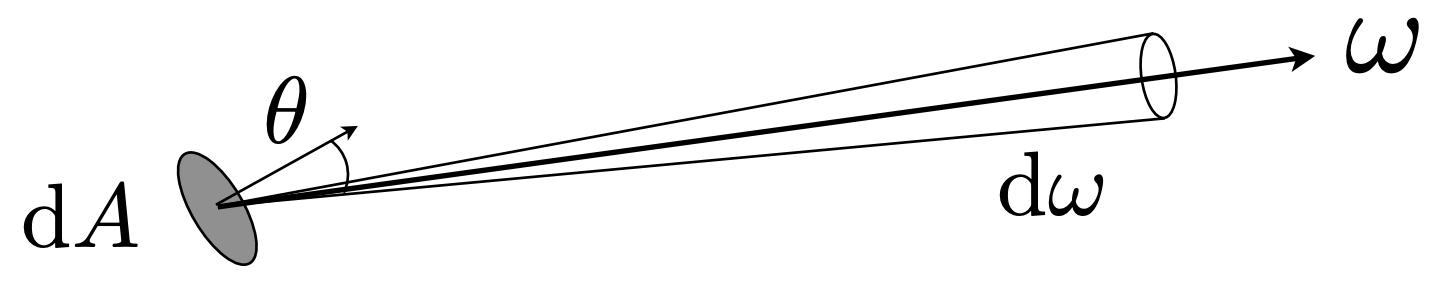
\includegraphics[scale=.25]{radiance.png}
	\caption{Radiance的计算}
	\label{fig:radiance}
\end{figure}

\begin{equation}
	L(p,\omega)=\frac{d^2\Phi(p,\omega)}{d\omega dA\cos\theta}
\end{equation} 单位是$\mathbf{W}/(\mathbf{sr}\cdot \mathbf{m}^2)$或者$\mathbf{nit}=\frac{\mathbf{lm}}{\mathbf{sr}\ \mathbf{m}^2}=\frac{\mathbf{cd}}{\mathbf{m}^2}$.我们可以从两个方面来理解Radiance. 从入射角度来说, 我们认为Radiance是单位立体角下的Irradiance: 
\begin{equation}
	L(p,\omega)=\frac{dE(p)}{d\omega \cos\theta}
\end{equation}

从出射的角度来说, 我们认为Radiance是单位面积下的Intensity: 
\begin{equation}
		L(p,\omega)=\frac{dI(p,\omega)}{dA \cos\theta}
\end{equation}

\section{Irradiance vs. Radiance}
\textbf{Irradiance}: 面积$dA$接收的所有能量

\textbf{Radiance}: 面积$dA$从指定\enquote{方向}$d\omega$接收到的能量

Irradiance也可以表示为Radiance在所有角度上的积分: 
\begin{equation}
	\begin{split}
		dE(p,\omega)=L_i(p,\omega)\cos\theta d\omega\\
		E(p)=\int_{H^2}L_i(p,\omega)\cos\theta d\omega
	\end{split}
\end{equation}我们只对上半球做积分, 我们认为和法线方向相反的光线对这一点没有贡献. 

\begin{figure}[H]
	\centering
	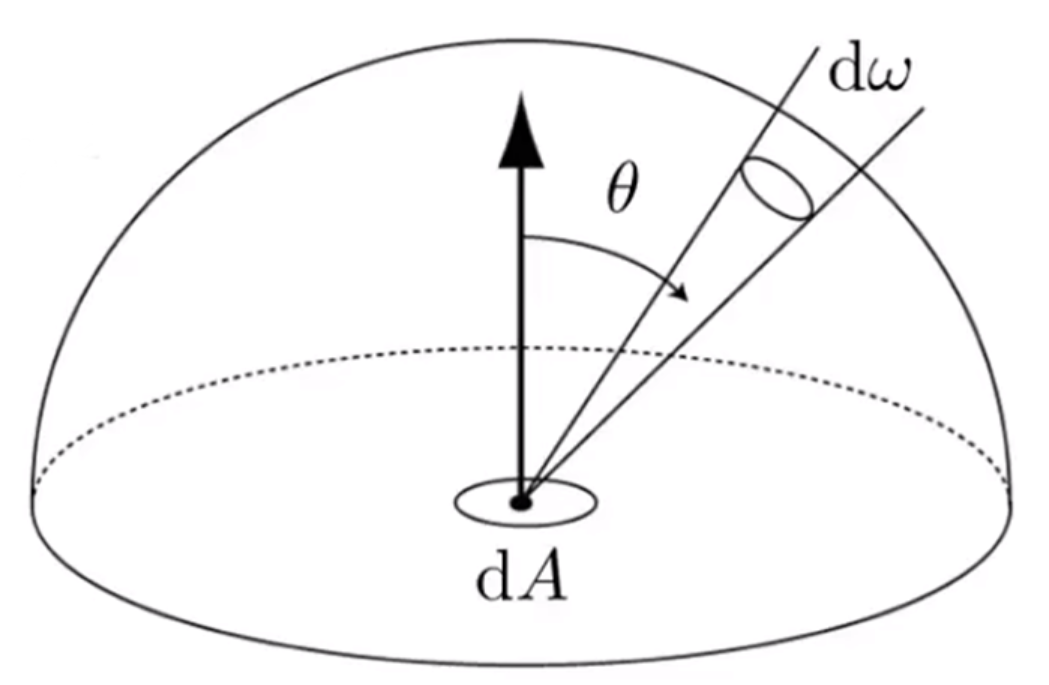
\includegraphics[scale=.4]{vs.png}
	\caption{Irradiance vs. Radiance}
	\label{fig:vs}
\end{figure}

\section{双向反射分布函数}
\textbf{双向反射分布函数 (Bidirectional Reflectance Distribution Fuction, BRDF) }定义了一个函数来表示从某一个角度入射的光线在某一个角度上会有多少能量被反射出去. 我们将反射的过程理解为两步: 第一步, 光线入射物体得到了一部分能量; 第二步, 物体将得到的能量再一次射出去. 

\begin{figure}[H]
	\centering
	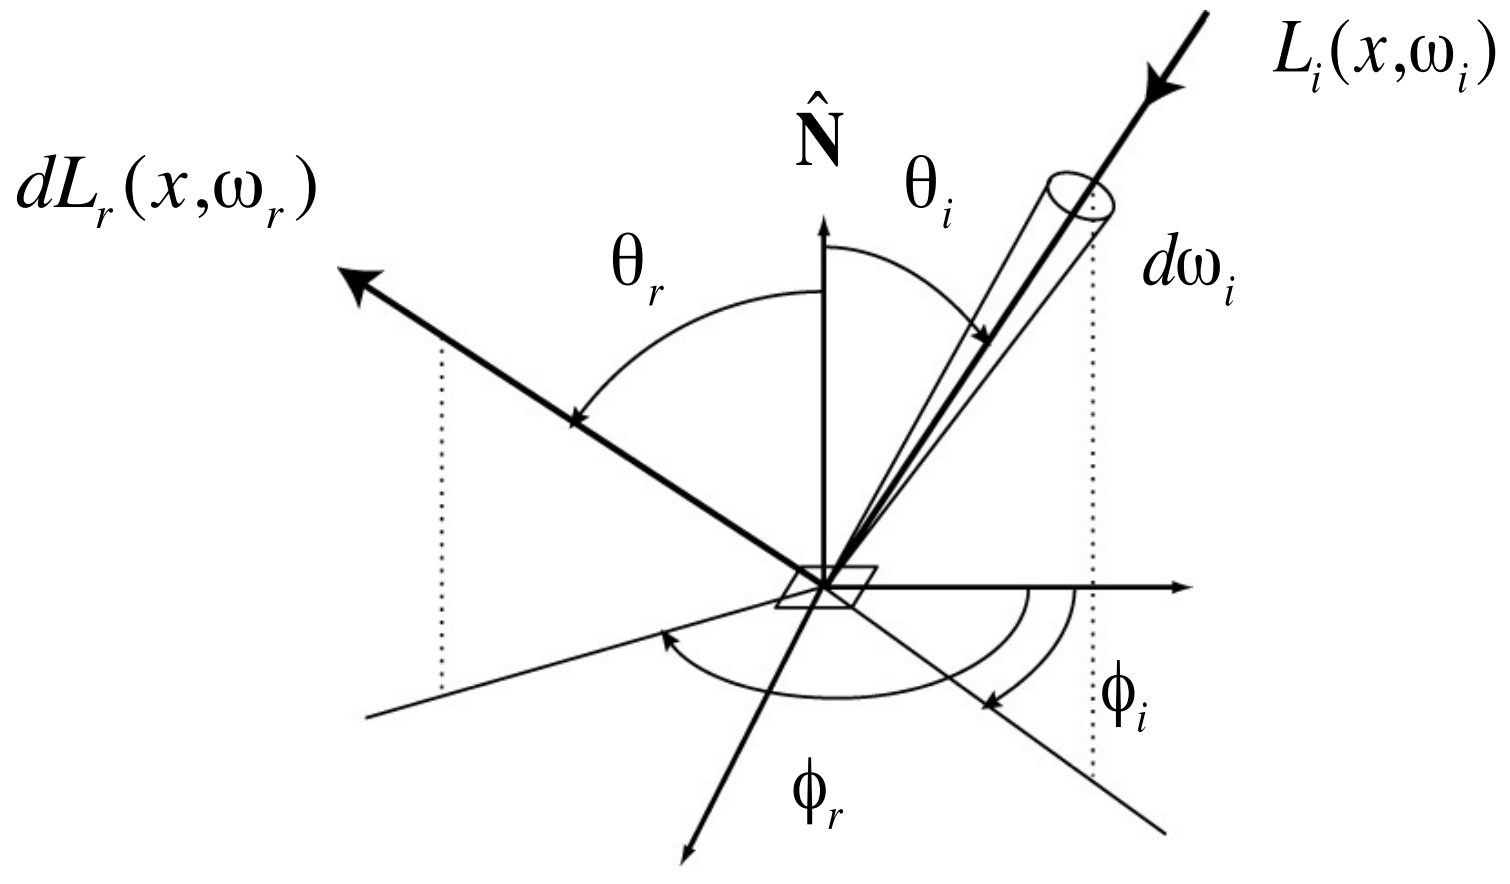
\includegraphics[scale=.35]{brdf.png}
	\caption{BRDF的定义}
	\label{fig:brdf}
\end{figure}

因此, 我们定义双向反射分布函数为: 
\begin{equation}
	f_r(\omega_i\rightarrow \omega_r)=\frac{dL_r(\omega_r)}{dE_i(\omega_i)}=\frac{dL_r(\omega_r)}{L_i(\omega_i)\cos\theta_i d\omega_i}[\frac{1}{sr}]
\end{equation}

那么, 对于某一个出射方向, 对应的能量应该是所有入射角度的光线反射结果的叠加: 
\begin{equation}
	L_r(p,\omega_r)=\int_{H^2}f_r(\omega_i\rightarrow \omega_r)L_i(p,\omega_i)\cos\theta_id\omega_i
\end{equation}

一个物体除了会反射来自其他物体的光线之外, 这个物体还有可能会自发光. 因此, 我们定义\textbf{渲染函数}为: 
\begin{equation}
	L_o(p,\omega_o)=L_e(p,\omega_o)+\int_{\Omega^+}L_i(p,\omega_i)f_r(p,\omega_i,\omega_o)(n\cdot \omega_i)d\omega_i
\end{equation}渲染函数包含两部分, 一部分是物体自发光, 另一部分是反射光. 在这里我们使用点乘代替$\cos\theta$计算. 我们的积分区域只在上半球, 法线反方向光线对于平面没有贡献. 

我们再一次理解这个公式, 我们可以认为$L_i$包含其他点光源, 面光源以及其他物体二次反射光线. 最终结果我们使用积分的方式进行叠加. 那么这个公式可以简写为: 
\begin{equation}
	I(u)=e(u)+\int I(v)K(d,v)dv
\end{equation} 我们可以通过矩阵再一次简化公式为: 
\begin{equation}
	l=E+KL
\end{equation}
通过求解矩阵我们可以得到: 
\begin{equation}
	L=(I-K)^{-1}E
\end{equation}

我们可以将矩阵进行展开, 可以得到: 
\begin{equation}
	\begin{split}
		L&=(1+K+K^2+K^3+\dots)E\\
		&=E+KE+K^2E+K^3E+\dots
	\end{split}
\end{equation}
每一项分别代表的是: 物体直接发出的光, 光源经过一次反射的光, 光源经过两次反射得到的间接光照, ……

\section{全局光照}
全局光照指的是直接光照以及间接光照的集合. 光栅化处理的是0次项和1次项的部分, 对于高阶项比较难处理. 随着我们不断叠加不同反射次数的结果, 图片会收敛到一个亮度, 不会一直变亮.

\chapter{蒙特卡洛路径追踪}

我们在上一节得到了渲染函数为
\begin{equation}
	L_o(p,\omega_o)=L_e(p,\omega_o)+\int_{\Omega^+}L_i(p,\omega_i)f_r(p,\omega_i,\omega_o)(n\cdot \omega_i)d\omega_i
\end{equation}
本节我们将通过数学工具求解这个函数并写成算法的形式来实现路径追踪. 

\section{蒙特卡洛积分}

对于任意一个函数, 不论是可以简单表达成解析式的还是不能轻松表达为解析式的函数, 我们都希望求出其定积分的结果. 在高等数学中我们使用\textbf{黎曼积分}求解. 也就是我们将曲线下的面积近似成一系列的小长方形的和. 当小长方形越多时, 得到的结果越相近. 

蒙特卡洛积分是通过多次随机采样并将采样对应的结果除以其概率密度的平均值作为积分结果. 也就是说对于一个采样概率分布$X_i\sim p(x)$, 蒙特卡洛积分为
\begin{equation}
	\int_a^b f(x) = F_N=\frac{1}{N}\sum_{i=1}^N\frac{f(X_i)}{p(X_i)}
\end{equation}

我们假设采样的概率分布是均匀分布, 也就是说$X_i\sim p(x)=\frac{1}{b-a}$, 那么蒙特卡洛积分可以表示为
\begin{equation}
	\int_a^b f(x) = F_N=\frac{b-a}{N}\sum_{i=1}^Nf(X_i)
\end{equation}

蒙特卡洛积分对于任何一种采样分布都是成立的. 只要进行采样就可以得到对应的积分. 使用蒙特卡洛积分要注意两点: 
\begin{enumerate}
	\item 采样的次数越多, 得到的结果越准确; 
	\item 采样必须在积分域上进行采样. 
\end{enumerate}

\section{路径追踪}
在之前的课程中我们介绍了Whitted-Style光线追踪, 但是这种追踪方式具有其极限性. Whitted-Style光线追踪仅计算光线的镜面反射, 因此对于某些弱于镜面反射的光线反射现象 (这里称作Glossy) 不能进行很好的表示. 因此我们选择使用渲染方程得到更加准确的求解. 

对于渲染函数我们有两个问题需要解决: 
\begin{enumerate}
	\item 我们需要求解积分项; 
	\item 这是一个递归的函数. 
\end{enumerate}

\subsection{积分求解}

使用蒙特卡洛积分求解积分项. 在这里我们限定仅计算来自光源的光线, 如果是来自其他物体的光线, 这里我们看作0.

我们和蒙塔卡洛积分进行对照, 发现$f(x)$对应的是$L_i(p,\omega_i)f_r(p,\omega_i,\omega_o)(n\cdot \omega_i)$. 积分域是$\omega_i$, $\omega_i$在上半球均匀分布采样的概率密度为$\frac{1}{2\pi}$. 

因此渲染函数的积分项可以写成: 
\begin{equation}
	\begin{split}
		L_o(p,\omega_o)&=\int_{\Omega^+}L_i(p,\omega_i)f_r(p,\omega_i,\omega_o)(n\cdot \omega_i)d\omega_i\\
		&\approx \frac{1}{N}\sum_{i=1}^{N}\frac{L_i(p,\omega_i)f_r(p,\omega_i,\omega_o)(n\cdot \omega_i)}{p(\omega_i)}
	\end{split}
\end{equation}

这样的过程我们可以写成伪代码的形式: 
\begin{lstlisting}[caption=渲染函数积分项对光源光线求解伪代码]
shade(p, wo)
	Randomly choose N directions wi~pdf
	Lo = 0.0
	For each wi
		Trace a ray r(p, wi)
		If ray r hit the light
			Lo += (1 / N) * L_i * f_r * cosine / pdf(wi)
	Return Lo
\end{lstlisting}

对于间接光照, 对于下图中的P点, 如果我们想要求出来自Q点的光线, 我们可以看作我们从P点看向Q点来自光源的光线反射得到的结果. 那么以上的伪代码我们可以改写为递归的形式: 


\begin{figure}[H]
	\centering
	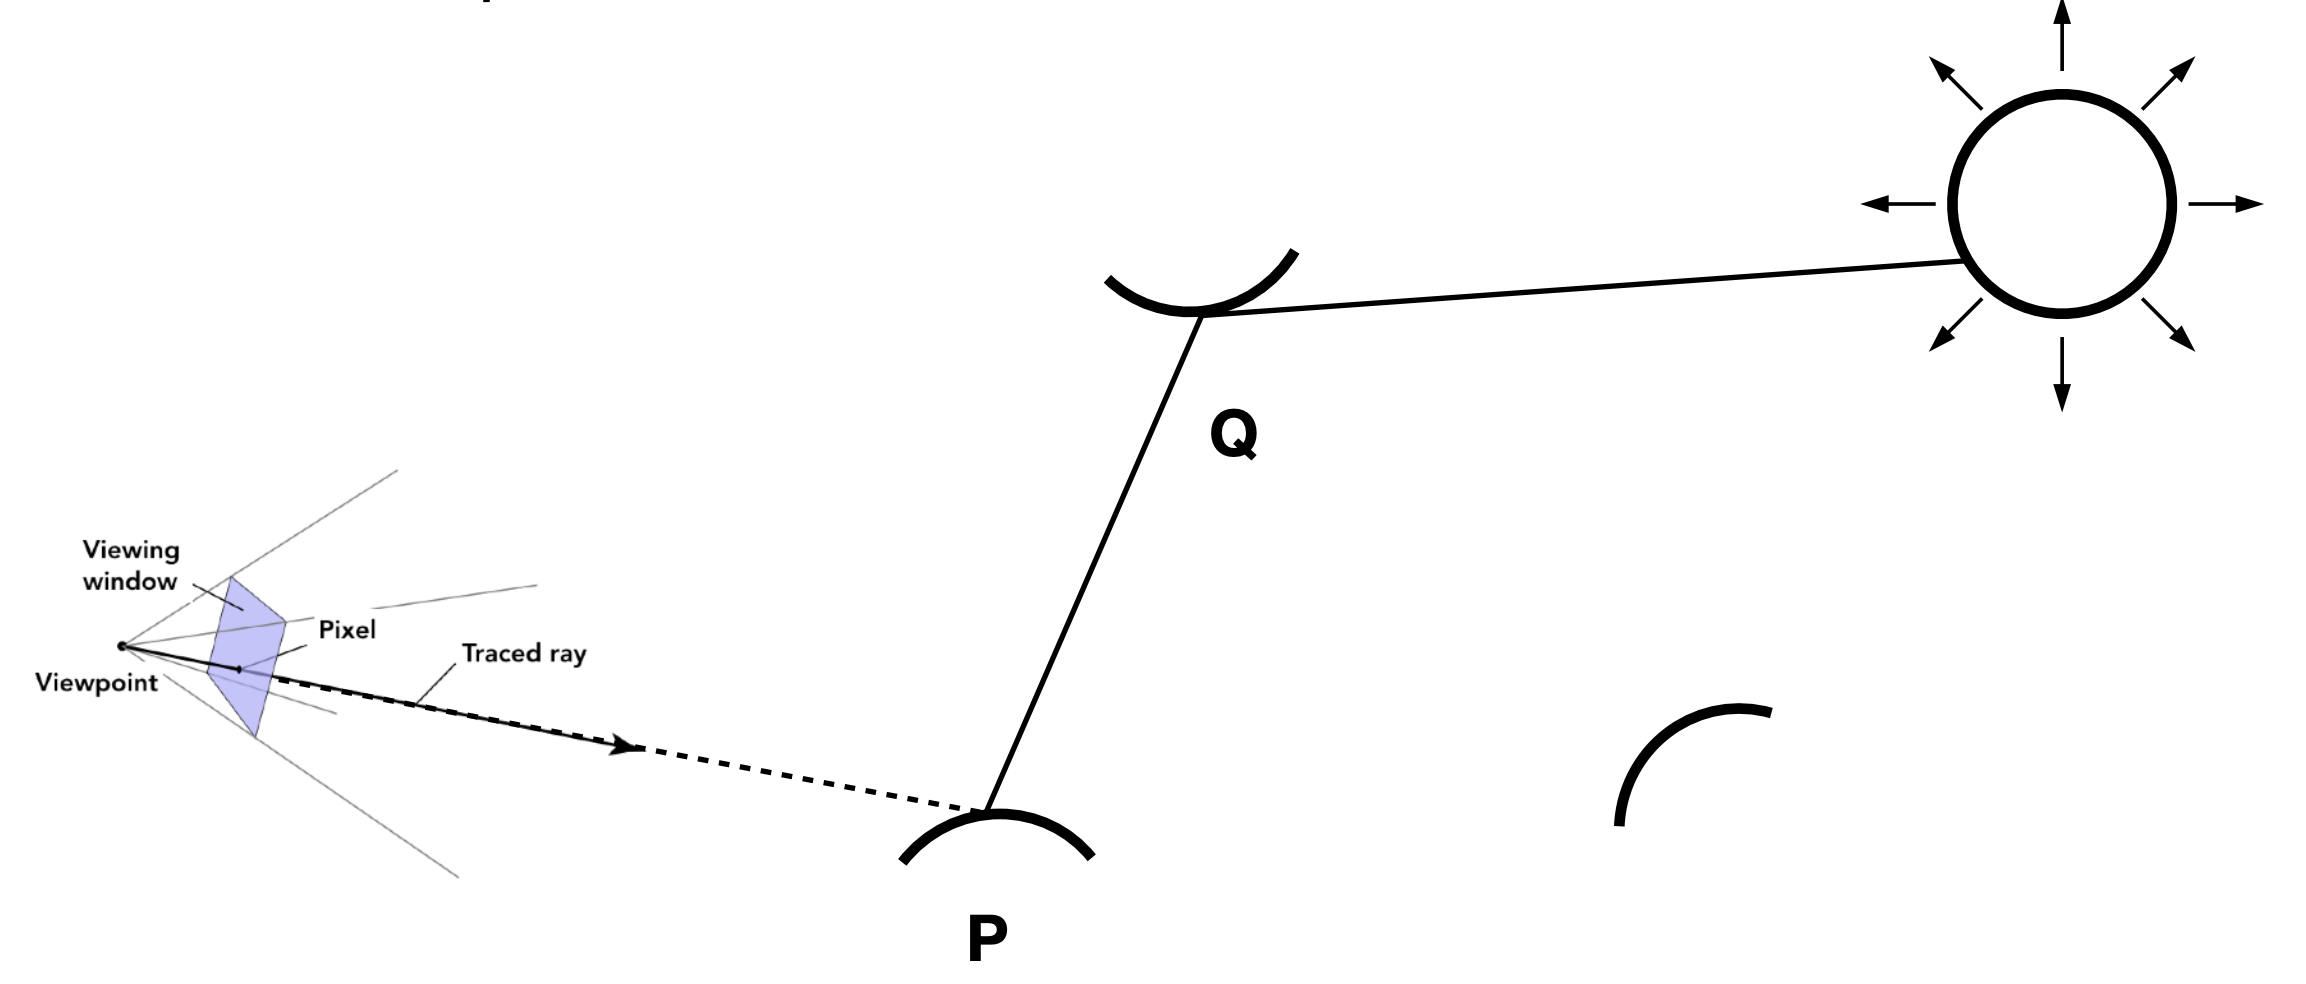
\includegraphics[scale=.25]{jianjieguangzhao.png}
	\caption{间接光照的递归求解}
	\label{fig:jjgz}
\end{figure}

\begin{lstlisting}[caption=渲染函数积分项的递归求解伪代码]
shade(p, wo)
	Randomly choose N directions wi~pdf
	Lo = 0.0
	For each wi
		Trace a ray r(p, wi)
		If ray r hit the light
			Lo += (1 / N) * L_i * f_r * cosine / pdf(wi)
		Else If ray r hit an object at q
			Lo += (1 / N) * shade(q, -wi) * f_r * cosine / pdf(wi)
	Return Lo
\end{lstlisting}

\subsection{算法优化}

\subsubsection{指数爆炸问题}

如果我们采样$N$次, 那么在经过$r$次反射后, 光线的数目可以达到$N^r$条, 会使计算量大大增加. 当且仅当$N=1$的时候, 不会产生指数爆炸问题. 此时我们转变方法, 在计算积分的时候我们仅计1次, 但是我们会在同一个像素中多次采样. 也就是说, 同一个像素上应该有多条光线通过, 我们对这些光线分别计算渲染函数后求平均就是这一像素的结果. 这个方法就是\textbf{路径追踪 (Path Tracing) }. 

\begin{lstlisting}[caption=渲染函数解决指数爆炸伪代码]
ray_generation(camPos, pixel)
	Uniformly choose N sample positions within the pixel
	pixel_radiance = 0.0
	For each sample in the pixel
		Shoot a ray r(camPos, cam_to_sample)
		If ray r hit the scene at p
			pixel_radiance += 1 / N * shade(p, sample_to_cam)
	Return pixel_radiance
\end{lstlisting}

\subsubsection{递归的停止问题}
我们的算法使用到了递归的方式. 但是我们的算法没有递归的结束条件. 因此我们需要引入一种方式结束递归. 我们引入俄罗斯轮盘赌 (RR) 的方式. 每一次光线都有$p$的概率能够反射出来. 如果说光线可以反射, 那么继续计算. 反之直接返回0.那么伪代码的形式是: 

\begin{lstlisting}[caption=包含递归停止条件的渲染函数伪代码]
shade(p, wo)
	Manually specify a probability P_RR
	Randomly select ksi in a uniform dist. in [0, 1]
	If (ksi > P_RR) return 0.0;
	 
	Randomly choose ONE directions wi~pdf
	Trace a ray r(p, wi)
	If ray r hit the light
		Return (1 / N) * L_i * f_r * cosine / pdf(wi) / P_RR
	Else If ray r hit an object at q
		Return (1 / N) * shade(q, -wi) * f_r * cosine / pdf(wi) / P_RR
\end{lstlisting}

我们返回的结果最终都会除以概率$p$, 这样子, 这一点得到结果的期望值和原来一样. 每一条光线反射次数的期望值是$\frac{p}{(1-p)^2}$.

\subsubsection{均匀分布并非最优解}

对于同一个点来说, 光源面积大, 那么我们使用较少的光线就可以接触到光源. 但是如果光源面积太小, 我们必须使用较多的光线才可以和光源发生接触. 那么对于小光源计算量会上升. 因此我们希望使用其他的概率分布进行采样, 使得采样得到的光线基本上都在光源上. 

我们的解决方案是在光源上进行均匀分布的采样, 这样子所有的光线一定都是来自于光源的. 

\begin{figure}[H]
	\centering
	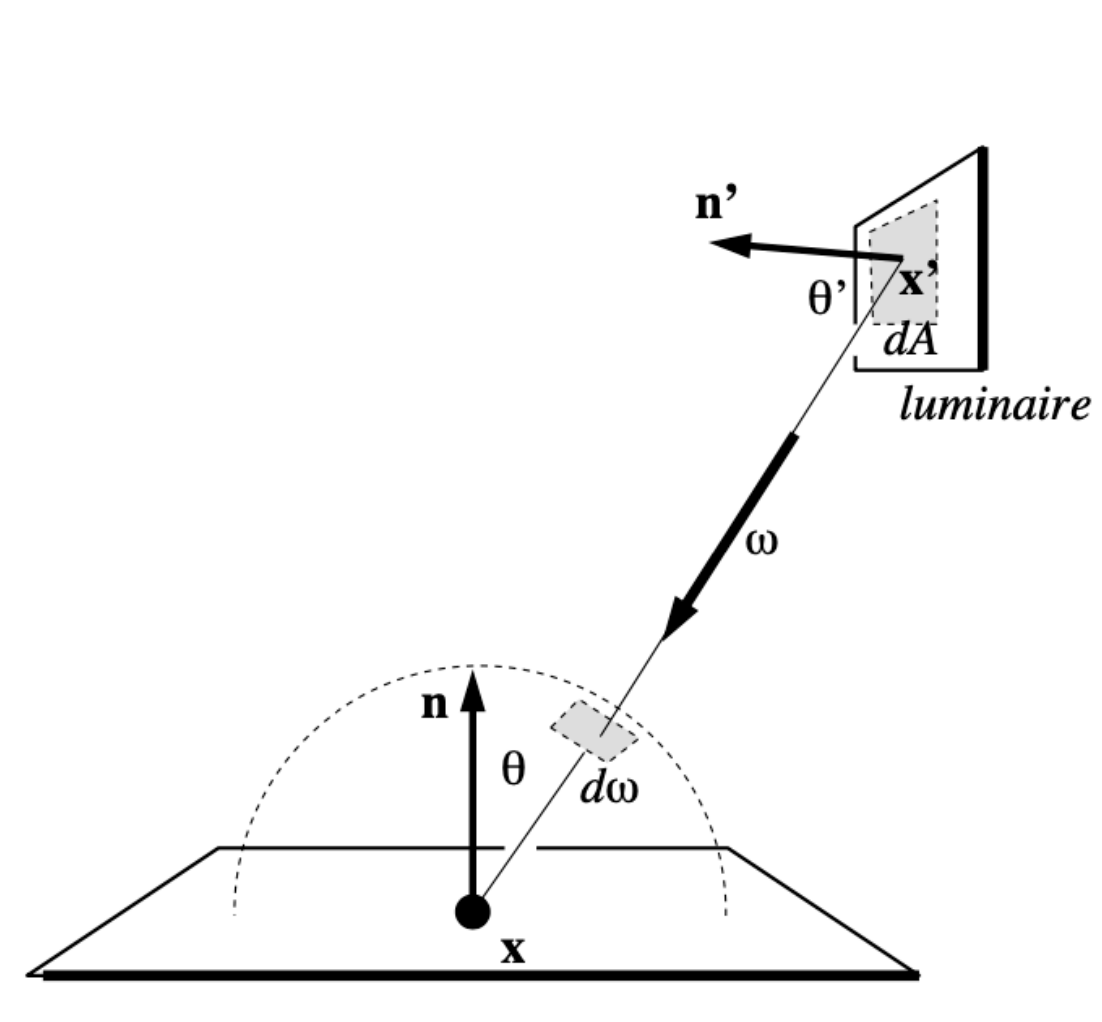
\includegraphics[scale=.25]{samplelight.png}
	\caption{从光源进行采样}
	\label{fig:samplelight}
\end{figure}

我们光源$A$上进行采样, 那么概率密度应该是$\frac{1}{A}$. 但是蒙特卡洛积分的采样必须在积分域上. 此时积分域发生了变换, 我们需要找到$d\omega$和$dA$之间的关系. $d\omega$是$dA$在对应单位球上的投影, 因此
\begin{equation}
	d\omega = \frac{dA\cos\theta'}{||x'-x||^2}
\end{equation}

那么积分式就可以改变为: 
\begin{equation}
	\begin{split}
		L_o(p,\omega_o)&=\int_{\Omega^+}L_i(p,\omega_i)f_r(p,\omega_i,\omega_o)\cos\theta d\omega_i\\
		&=\int_AL_i(p,\omega_i)f_r(p,\omega_i,\omega_o)\frac{\cos\theta\cos\theta'}{||x'-x||^2}dA
	\end{split}
\end{equation}

此时, 我们需要更改一下之前RR的策略. 对于直接光照, 不使用RR; 对于间接光照使用RR. 这样我们就把问题分为了两部分——直接光照和间接光照. 

\begin{lstlisting}[caption=采用光源上均匀分布渲染函数伪代码]
shade(p, wo)
	# Contribute from the light source
	Uniformly sample the light at x' (pdf_light = 1 / A)
	L_dir = L_i * f_r * cos(theta) * cos(theta') / |x' - p| ^ 2 / pdf_light
	
	# Contribute from other reflectors
	L_indir = 0.0
	Test Rassian Roulette with probability P_RR
	Uniformly sample the hemisphere toward wi (pdf_hemi = 1 / 2pi)
	Trace a ray r(P, wi)
	If ray r hit a non-emitting object at q
		L_indir = shade (q, -wi) * f_r * cos(theta) / pdf_hemi / P_RR
	
	Return L_dir + L_indir
\end{lstlisting}

最后我们只需要对光源和反射点间有物体的情况进行判断即可, 

\begin{lstlisting}[caption=渲染函数伪代码]
	shade(p, wo)
	# Contribute from the light source
	L_dir = 0.0
	Uniformly sample the light at x' (pdf_light = 1 / A)
	Shoot a ray from p to x'
	If the ray is not blocked in the middle
		L_dir = L_i * f_r * cos(theta) * cos(theta') / |x' - p| ^ 2 / pdf_light
	
	# Contribute from other reflectors
	L_indir = 0.0
	Test Rassian Roulette with probability P_RR
	Uniformly sample the hemisphere toward wi (pdf_hemi = 1 / 2pi)
	Trace a ray r(P, wi)
	If ray r hit a non-emitting object at q
	L_indir = shade (q, -wi) * f_r * cos(theta) / pdf_hemi / P_RR
	
	Return L_dir + L_indir
\end{lstlisting}

这样我们就得到了最终路径追踪的算法. 


\chapter{材质和外观}

\textbf{材质和外观 (Material and Appearance) }是渲染物体非常重要的属性之一. 光线的传播和材质具有密切的关系. 

\section{材质的定义}

在渲染函数中, 我们分析各个参数可以知道材质和双向反射分布函数 (BRDF) 具有密切的关系. BRDF决定了物体的材质属性. 接下来我们将对三种不同的材质定义其对应的BRDF. 

\begin{figure}[H]
	\centering
	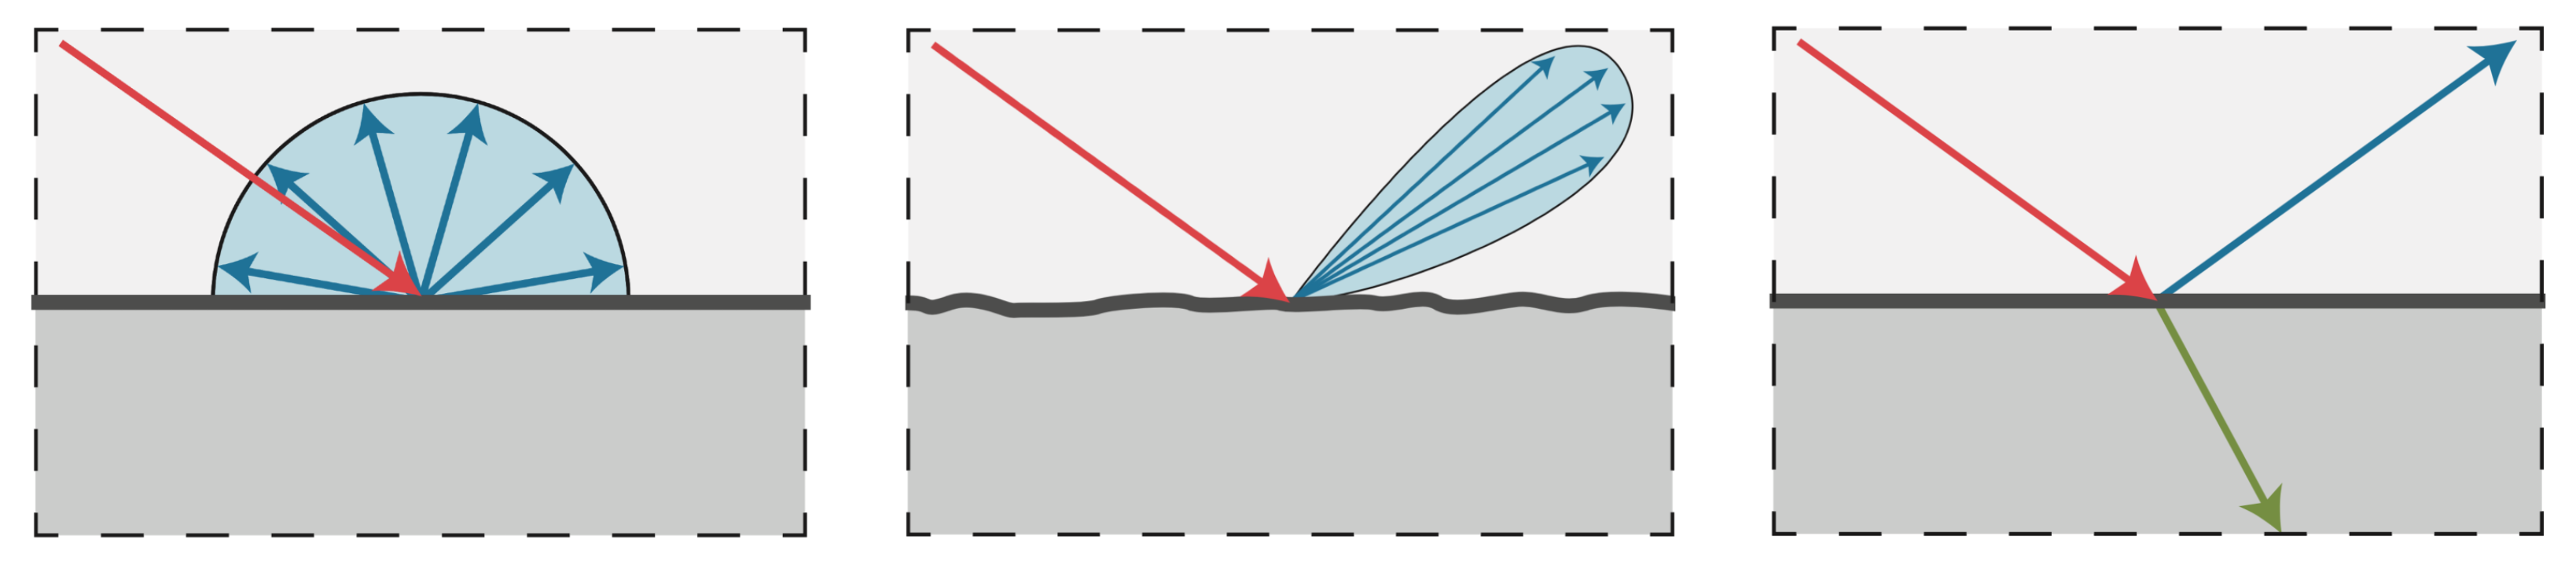
\includegraphics[scale=.35]{material.png}
	\caption{从左到右: 漫反射材质, 光泽表面材质以及折射材质}
	\label{fig:material}
\end{figure}

\subsection{漫反射材质}
\textbf{漫反射材质 (Diffuse / Lambertian Material) }的性质是当一束光线从任意方向射向材质表面时, 将会向各个方向均匀的反射光. 

对于任何一个出射角$\omega_o$, 对应的Radiance的大小为: 
\begin{equation}
	\begin{split}
		L_o(\omega_o)&=\int_{H^2}f_rL(\omega_i)\cos\theta_id\omega_i\\
		&=f_rL_i\int_{H^2}cos\theta_id\omega_i\\
		&=\pi f_r Li
	\end{split}
\end{equation}
根据能量守恒定律, $L_o=L_i$, 因此我们可以得到$f_r=\frac{1}{\pi}$. 我们引入一个反射率 (Albedo) $\rho$反应能量的衰减: 
\begin{equation}
	f_r=\frac{\rho}{\pi}
\end{equation}
反射率既可以是一个通道对能量的衰减, 也可以在RGB空间上定义一个三维的反射率来表示颜色. 

\section{光泽表面材质和折射材质}

\textbf{光泽表面材质 (Glossy material ) }一般表示的是金属材质. 这些材质相比于镜面来说没有那么光滑, 但是依然可以产生非常类似于镜面反射的效果 (光线的出射方向非常的集中) . 

\textbf{折射材质 (Ideal reflective / refractive material) } 可以折射一定量的光线. 这种材质通常是透明材质, 例如玻璃或者水. 

\section{散射定律}

\subsection{反射定律}

\textbf{反射定律 (Reflection Law) }指光射到一个界面上时, 其入射光线与反射光线成相同角度. 我们用数学方法定义在立体角上的反射定律: 

\begin{figure}[H]
	\centering
	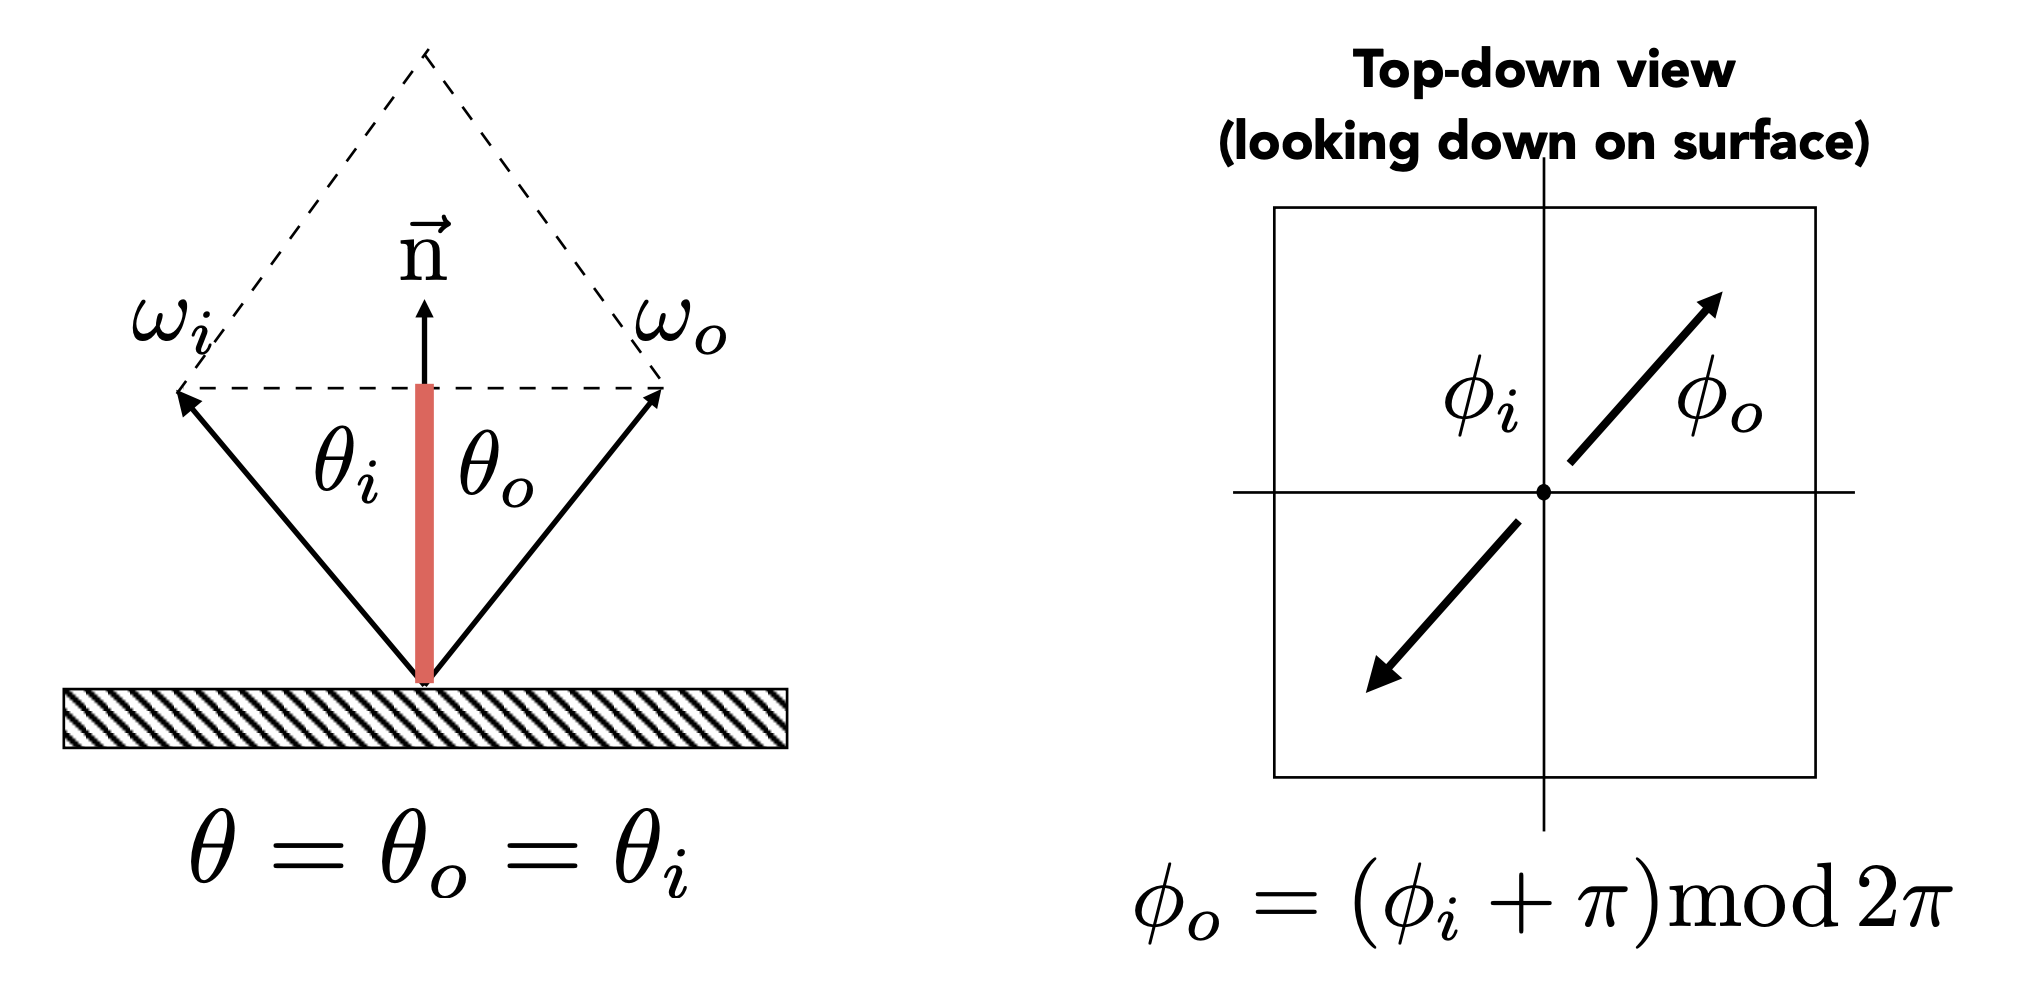
\includegraphics[scale=.25]{fanshe.png}
	\caption{反射定律}
	\label{fig:fanshed}
\end{figure}

在光线和法线所在的平面上, 反射角等于入射角, 也就是说$\theta=\theta_o=\theta_i$.如果我们垂直于法线观测, 入射光线和反射光线方向完全相反, 也就是$\phi_o=(\phi+\pi)\mod 2\pi$.

根据反射定律, 我们在知道入射角和法线方向的时候就可以求出出射角方向: 
\begin{equation}
	\begin{split}
		&\because \omega_o + \omega_i = 2\cos\theta \overrightarrow{n} = 2(\omega_i\cdot \overleftarrow{n})\overrightarrow{n}\\
		&\therefore \omega_o = -\omega_i + 2(\omega_i\cdot \overrightarrow{n})\overrightarrow{n}
	\end{split}
\end{equation}

\subsection{折射定律}

\textbf{折射定律 (Snell's Law) }反映了折射角和入射角的关系. 

\begin{figure}[H]
	\centering
	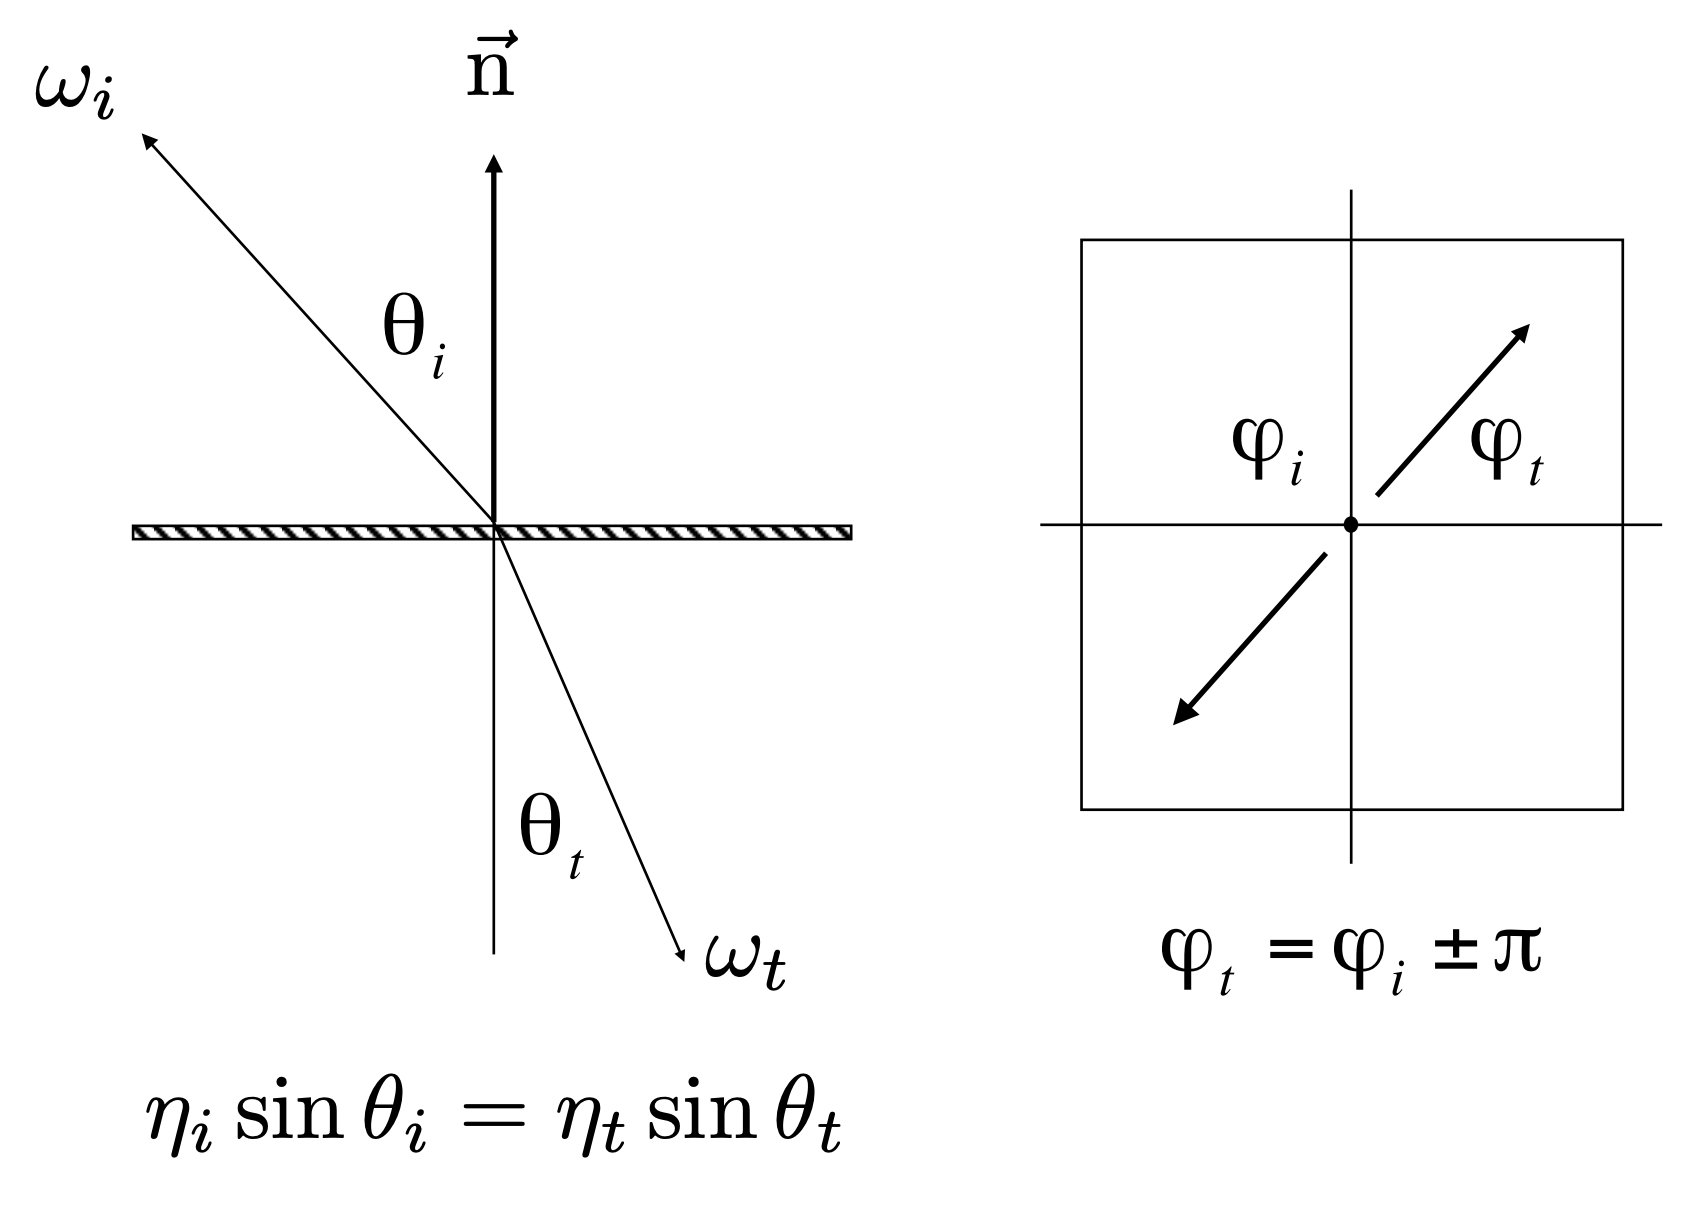
\includegraphics[scale=.25]{zheshe.png}
	\caption{折射定律}
	\label{fig:zheshe}
\end{figure}

根据折射定律, 在光线和法线所在平面上, 折射率和光线于法线的夹角正弦值相等. 也就是说: 
\begin{equation}
	\eta_i\sin\theta_i = \eta_t=\sin\theta_t
\end{equation}
其中$\eta$是这种材质的折射率. 垂直于法线观测的情况和反射定律相同, 两条光线方向是相反的. 

常见的材质的折射率如下表所示: 

\begin{table}[H]
	\centering
	\begin{tabular}{cl}
		\hline
		材质       & $\eta$  \\ \hline
		真空       & 1.0     \\
		空气 (海平面)   & 1.00029 \\
		水 (20摄氏度)  & 1.333   \\
		玻璃       & 1.5-1.6 \\
		钻石       & 2.42  \\ \hline
	\end{tabular}
	\caption{常见材质的折射率}
\end{table}

根据折射定律, 我们在知道入射角和法线方向以及材质的折射率的时候就可以求出出射角方向: 
\begin{equation}
	\begin{split}
		\cos\theta_t&=\sqrt{1-\sin^2\theta_t}\\
		&=\sqrt{1-(\frac{\eta_i}{\eta_t})^2\sin^2\theta_i}\\
		&=\sqrt{1-(\frac{\eta_i}{\eta_t})^2(1-\cos^2\theta_i)}
	\end{split}
\end{equation}

我们对以上公式进行讨论. 当根号下的结果如果小于0, 当且仅当$\frac{\eta_i}{\eta_t}>1$.也就是说当入射介质的折射率大于反射介质的折射率时, 就有可能发生\textbf{全反射}现象. 

\section{菲涅耳项}

在现实生活中, 我们发现这样的现象. 当我们在不同的视角下进行观察的时候会用不同的现象. 如下图所示, 当我们从不同的视角观察桌子的时候, 桌子对书反射的程度也不尽相同. 这就是菲涅耳带来的结果. 

\begin{figure}[H]
	\centering
	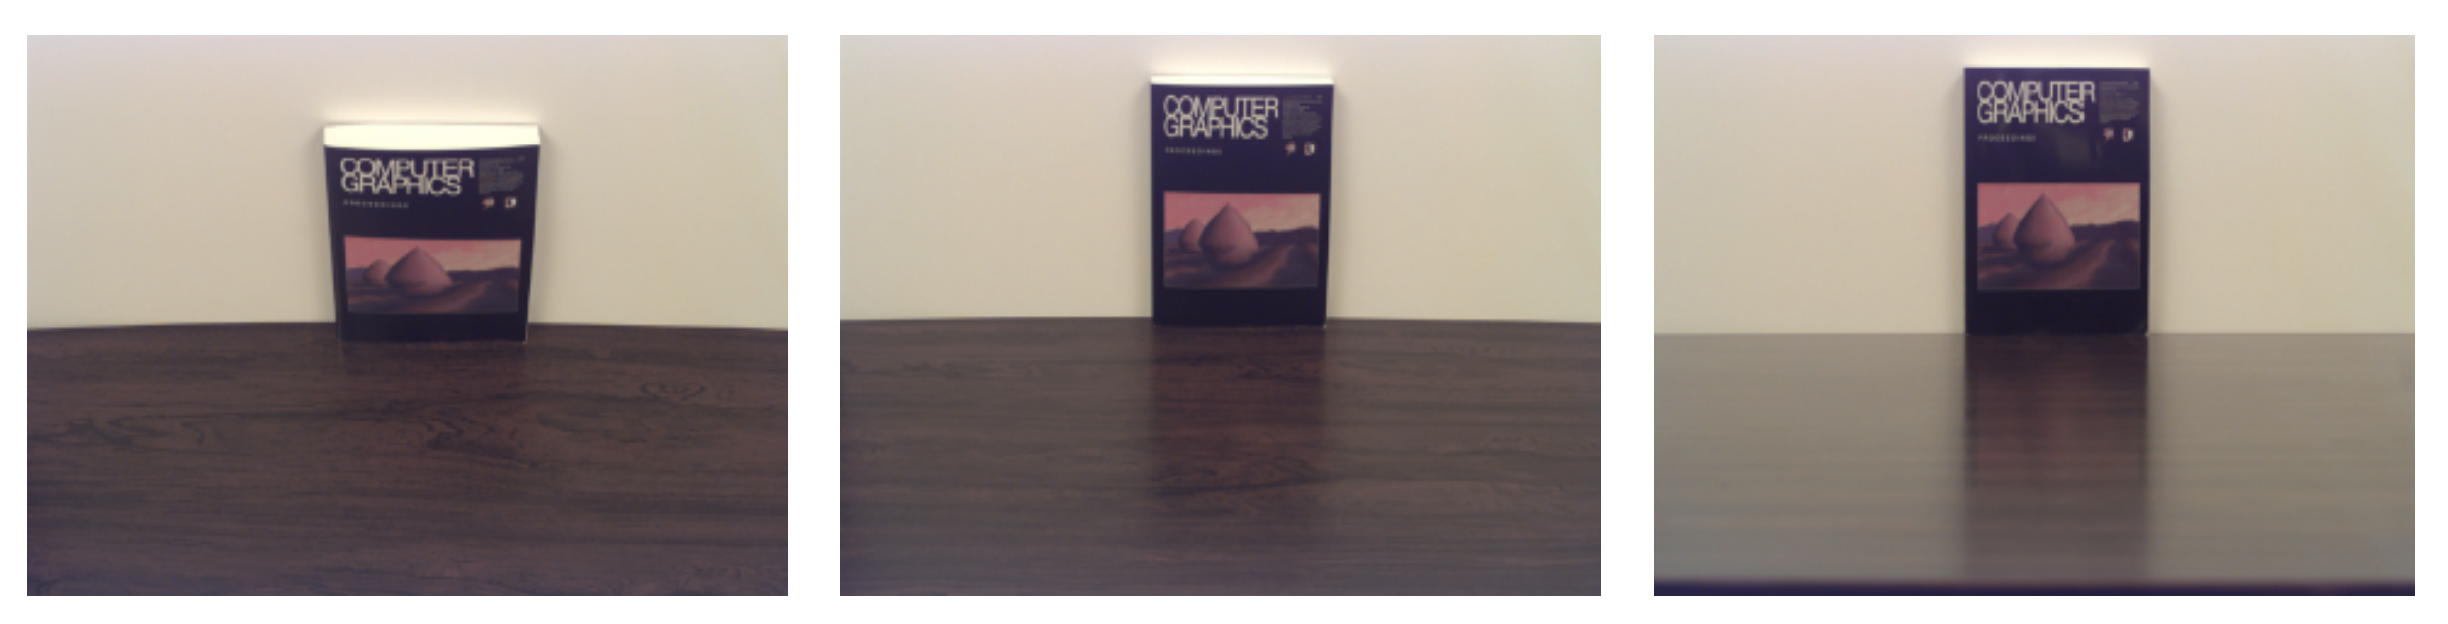
\includegraphics[scale=.25]{feinieer.png}
	\caption{菲涅耳项带来的现象}
	\label{fig:fne}
\end{figure}

对于导体和非导体, 菲涅耳项满足: 
\begin{itemize}
	\item 对于非导体, 入射光线和入射平面越近, 被反射出去的光线越多; 
	\item 对于导体, 反射出来光线的多少和入射角度没有直接关系, 光线都可以被大量反射出去. 
\end{itemize}

菲涅耳项的准确计算方法是: 
\begin{equation}
	\begin{split}
		R_s&= \lvert\frac{n_1\cos\theta_i-n_2\cos\theta_t}{n_1\cos\theta_i+n_2\cos\theta_t}\rvert^2 = \lvert{\frac{n_1\cos\theta_i-n_2\sqrt{1-(\frac{n_1}{n_2}\sin\theta_i)^2}}{n_1\cos\theta_i+n_2\sqrt{1-(\frac{n_1}{n_2}\sin\theta_i)^2}}}\rvert^2\\
		R_p&= \lvert\frac{n_1\cos\theta_t-n_2\cos\theta_i}{n_1\cos\theta_t+n_2\cos\theta_i}\rvert^2 = \lvert{\frac{n_1\sqrt{1-(\frac{n_1}{n_2}\sin\theta_i)^2}-n_2\cos\theta_i}{n_1\sqrt{1-(\frac{n_1}{n_2}\sin\theta_i)^2+n_2\cos\theta_i}}}\rvert^2\\
		R_{eff}&=\frac{1}{2}(R_s+R_p)
	\end{split}
\end{equation}
其中, $R_s$和$R_p$是在s极点和p极点的菲涅耳项, 我们使用他们的平均作为我们使用的菲涅耳项. 但是这种计算方式过于的复杂, 因此还提供了一种比较简单的菲涅耳项计算方法: 
\begin{equation}
	\begin{split}
		R(\theta)&=R_0+(1-R_0)(1-\cos\theta)^5\\
		R_0&=(\frac{n_1-n_2}{n_1+n_2})^2
	\end{split}
\end{equation}

\section{微表面模型}

\textbf{微表面模型 (Microfacet Material) }是更接近于物理的材质描述. 我们认为\textbf{广表面 (Macrosurface) }是平坦且粗糙的, 但是\textbf{微表面 (Microsurface) }是凹凸不平但是光滑的 (每一个小的面都是光滑平坦的) . 那么整体的光线反射情况应当是所有微表面反射情况的总和. 从近处看是几何, 从远处看就是一种材质. 

对于任何一种材质, 我们使用法线分布来描述其材质. 如果是光滑的表面, 那么法线分布比较集中; 否则, 法线会分布在四处. 在微表面的情况下BDRF可以写作: 
\begin{equation}
	f(i,o)=\frac{F(i,h)G(i,o,h)D(h)}{4(n,i)(n,o)}
\end{equation}
其中, $F(\cdot)$是菲涅耳项, $D(h)$是沿着半向量 (Half Vector, $h=\frac{1}{2}(i+o)$) 方向的法线分布. $G(\cdot)$是一个几何项, 微表面内部可能会有几何遮挡, 使一些微表面失去了作用. 自遮挡容易发生在几乎和反射面平行入射的方向 (Grazing angle) . 分号下的两项是推倒项. 

\section{材质的分类}

本节我们将材质根据法线的分布进行分类, 分别是: 
\begin{itemize}
	\item 各向同性材质 (Isotropic Material) : 各个方向上法线分布一致的材质, 满足$f_r(\theta_i,\phi_i;\theta_r,\phi_r)=f_r(\theta_i,\theta_r,\phi_r-\phi_i)$; 
	\item 各向异性材质 ( Anisotropic Material) : 各个方向上法线分布不一致的材质, 满足足$f_r(\theta_i,\phi_i;\theta_r-\phi_r)\neq f_r(\theta_i,\theta_r,\phi_r,-\phi_i)$, 常见于打磨过的金属, 尼龙材料. 
\end{itemize}

\section{BRDF的性质}
\begin{itemize}
	\item 非负性
	\begin{equation}
		f_r(\omega_i\rightarrow \omega_o) \geq 0
	\end{equation}
	\item 线性可加
	\item 可逆性
	\begin{equation}
		f_r(\omega_i\rightarrow \omega_o)=f_r(\omega_o\rightarrow \omega_i)
	\end{equation}
	\item 能量守恒
	\begin{equation}
		\forall\omega_r\ \int_{H^2}f_r(\omega_i\rightarrow \omega_o)\cos\theta_id\omega_i\leq 1
	\end{equation}
	\item 各向同性材质的特别性质
	\begin{equation}
		f_r(\theta_i,\theta_r,\phi_r-\phi_i)=f_r(\theta_r,\theta_i,\phi_i-\phi_r)=f_r(\theta_i,\theta_r,|\phi_r-\phi_i|)
	\end{equation}
\end{itemize}

\section{BRDF的测量}

我们希望准确的测量出真实世界材质的BDRF. 如下图所示, 我们可以通过以下的实验方式测量某一种材质的BDRF. 

\begin{figure}[H]
	\centering
	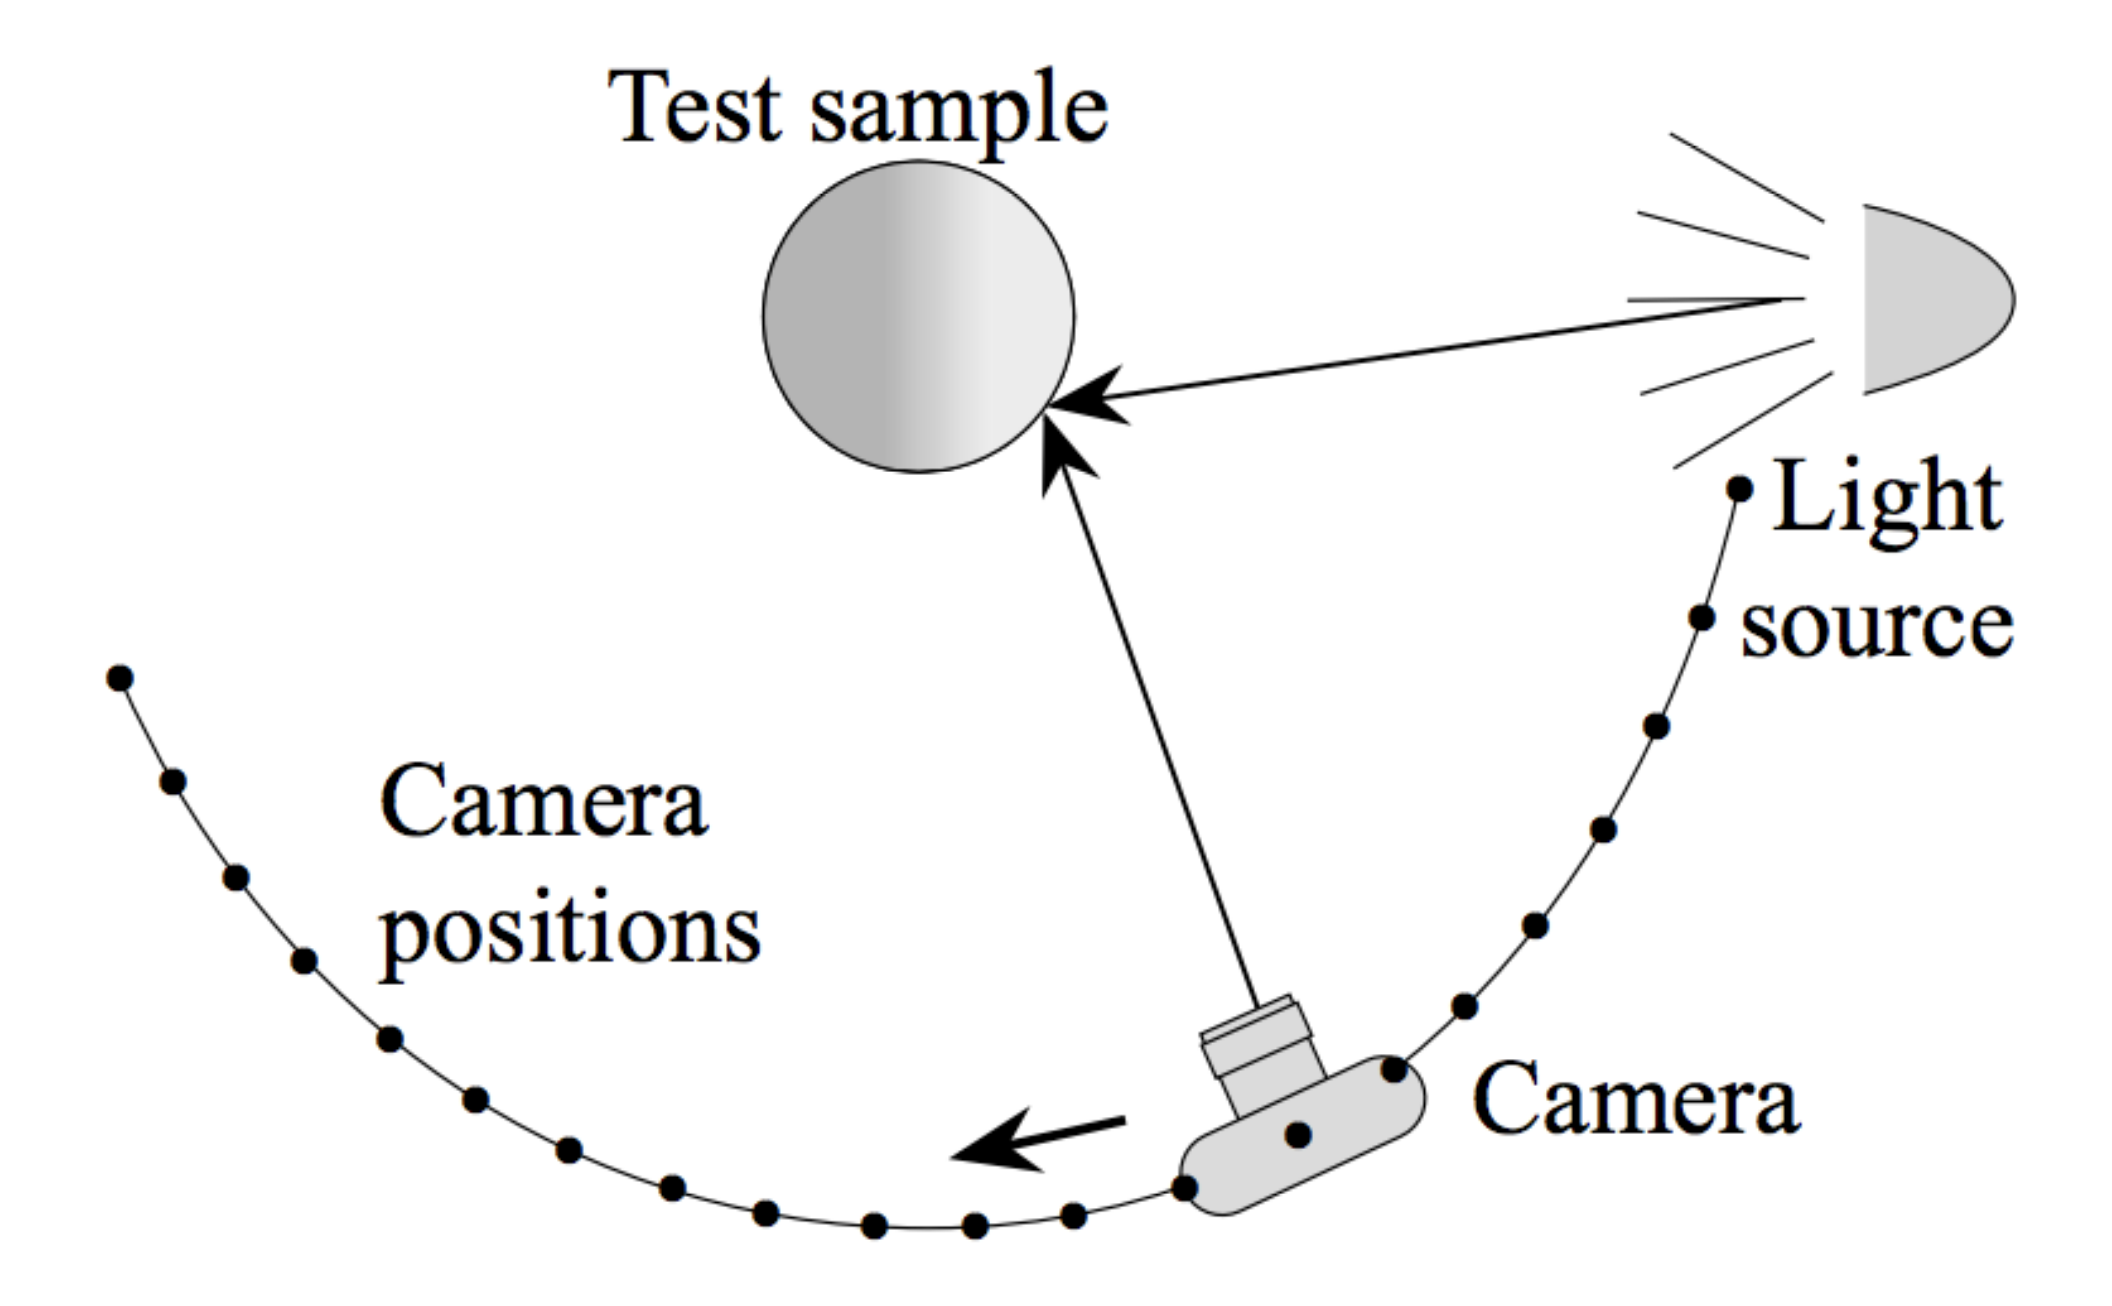
\includegraphics[scale=.25]{bdfrce.png}
	\caption{测量材质的BDRF}
	\label{fig:bdrfce}
\end{figure}

我们可以通过这样的装置得到各个入射方向和出射方向的BDRF, 测量的算法如下: 
\begin{lstlisting}[caption=BDRF的测量]
foreach outgoing direction wo
	move light to illuminate surface with a thin beam from wo
	for each incoming direction wi
		move sensor to be at direction wi from surface
		measure incident radiance
\end{lstlisting}

这样的测量方式是需要使用四维的参数. 但是如果我们测量的是各向同性材质, 参数可以降至三维. 又因为可逆性, 我们只需要测量一半的情况就可以. MERL BRDF Database就是一个包含了各种材质BRDF的数据库. 

\chapter{高级渲染理论}

\section{高级光线传播 (Advanced Light Transport) }

\subsection{有偏与无偏蒙特卡洛估计}

\textbf{有偏 (Biased) }蒙特卡洛估计指的是如果我们取样后得到的估计值与要预测的真实值是有偏差的, 那么我们认为这是一个有偏估计. 当我们采样足够大的的时候, 有偏估计也可以收敛到正确值, 这说明了有偏估计具有一致性. \textbf{无偏 (Unbiased) }蒙塔卡洛估计指的是不论我们选取多少样本进行估计, 得到的期望值和正确值一样. 

\subsection{双向路径追踪}

\textbf{双向路径追踪 (Bidirectional Path Tracing, BDPT) }指的是我们分别从光源和眼睛 (摄像机) 引出半路径, 并将半路径的终点连接起来形成路径. 这种方法非常适用于光源出光线比较复杂的情况. 但是实现困难并且渲染比较慢, 是一种无偏的估计. 

\begin{figure}[H]
	\centering
	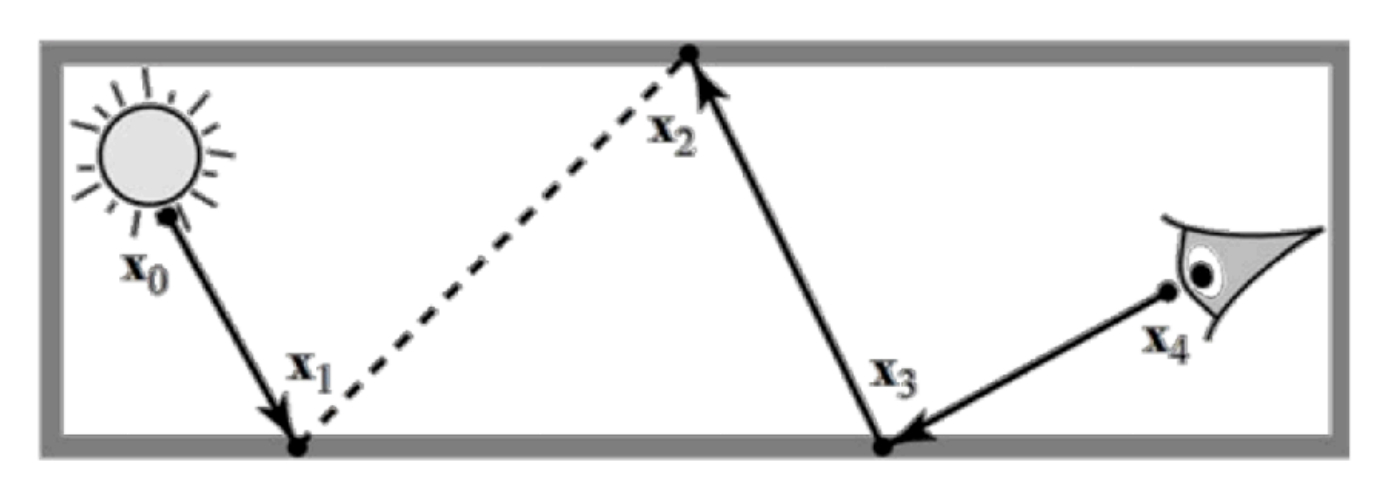
\includegraphics[scale=.25]{bdpt.png}
	\caption{双向路径追踪}
	\label{fig:bdpt}
\end{figure}

\subsection{Metropolis 光线传播}

\textbf{Metropolis光线传播 (Metropolis Light Transport, MLT) }使用马尔可夫链的方法进行采样. 这种采样方式可以很容易的采样到某一个采样的临近点. 其主要思想是, 当一条路径可以到达光源时, 那么临近的采样也应该容易到达光源. 非常适用于困难场景的渲染, 尤其是SDS (Specular-Diffuse-Specular) 路径. 但是很难估计收敛速度, 每一个像素的收敛速度也不一样. 操作独立, 各个像素独立导致画面会比较``脏”, 因此很难应用到动画上. 同样, 这可以无偏估计. 

\subsection{光子映射}

\textbf{光子映射 (Photon Mapping) }是一个分为两步的方法. 是一种有偏估计. 适合于SDS路径以及焦散材质. 
\begin{enumerate}
	\item 从光源出发射出光子, 当光子反射到漫反射平面时停止, 记录光子位置; 
	\item 从摄像机射出半路径, 直到路径反射到漫反射平面上. 
\end{enumerate}

我们需要通过局部密度估计在计算单位面积内, 光子数的多少. 那么光子密度越高的地方应当越亮. 对于任意一个点, 我们选取临近$N$个距离最近的光子, 那么使用$N$处以光子所占的面积$\triangle A$就可以得到该点的局部密度. 

\begin{figure}[H]
	\centering
	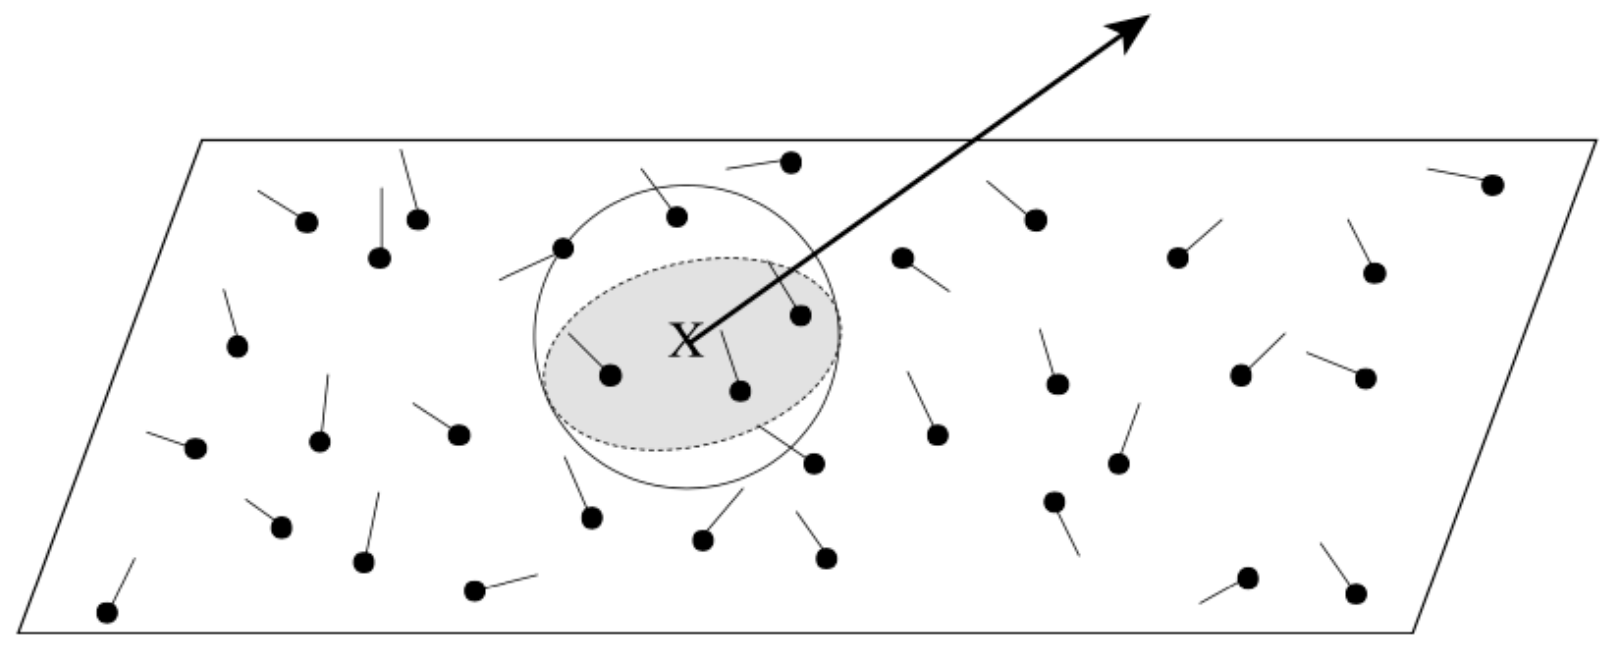
\includegraphics[scale=.25]{mlt.png}
	\caption{光子的局部密度估计}
	\label{fig:mlt}
\end{figure}

为什么这是一个有偏的方法?我们$N$太少的话易产生噪声, 但是$N$太多又会模糊. 当我们使用的光子足够多的时候, $\triangle A$就趋近于$\text{d}A$.因此, 只要我们的采样是有限的, 得到的密度多少都会有偏差, 所以这是一个有偏的估计. 但是这是一致的估计. 

\subsection{VCM}

\textbf{Vertex Connection and Merging (VCM)}是一种结合了双向路径追踪和光子映射的方法. 其主要思想是在双向光线追踪中如果半路径的结束点并不在一起但是距离比较近的话可以组合在一起. 使用光子映射的方法来组合这些临近的``光子”. 是一种有偏估计. 

\subsection{实时辐射度}

\textbf{实时辐射度 (Instant Radiosity, IR) }最主要的思想是认为被照亮的表面可以当作一个小光源. 从光源打出来的地方到一些表面后, 到达点就是新的虚拟光源. 之后就可以将这些虚拟光源看作光源进行渲染. 优点是渲染速度快并且在漫反射场景中表现的很好. 缺点是不能很好的处理反射材质. 

\section{高级外观建模}

\subsection{非表面模型}

\subsubsection{散射介质}

对于一些\textbf{散射介质 (Participating media) }, 例如云、雾, 我们认为他们是非表面模型. 因此他们不存在一个表面, 而是由许多散射小颗粒组成的. 任何一束光通过散射介质, 会发生 (部分) 吸收或者散射. 

\begin{figure}[H]
	\centering
	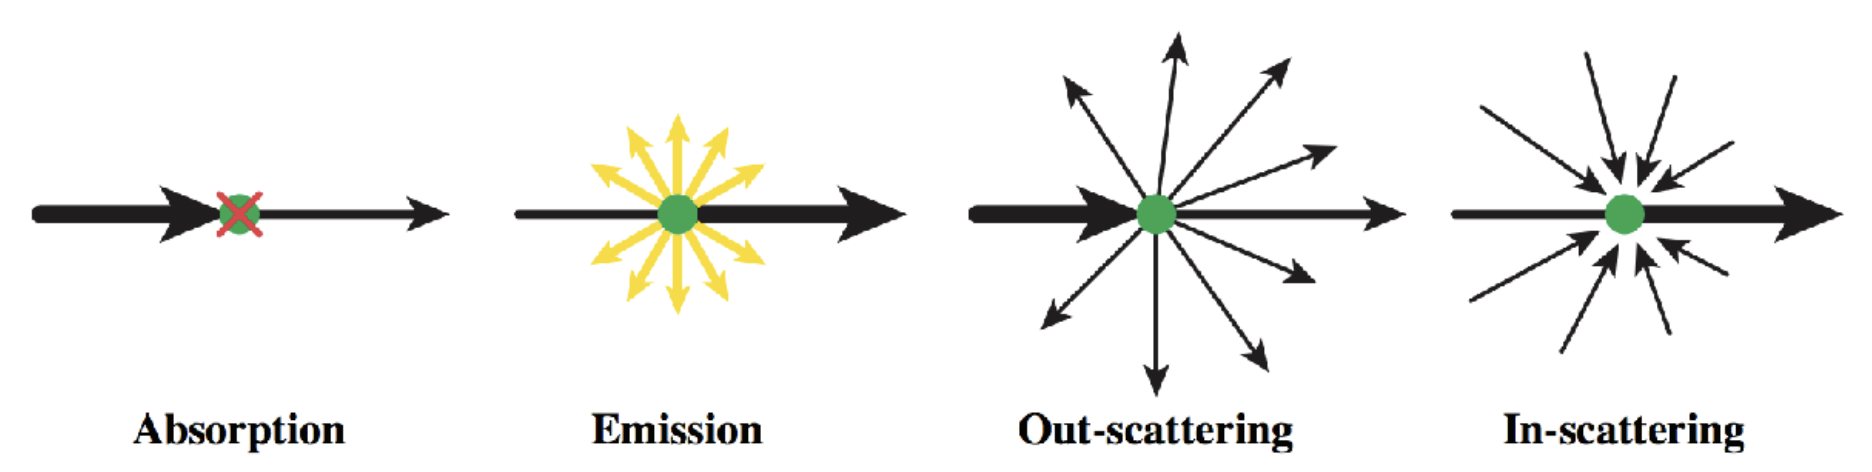
\includegraphics[scale=.35]{pm.png}
	\caption{散射介质的吸收, 发光, 外散射和内散射}
	\label{fig:pm}
\end{figure}

我们采用相位函数去描述在某一点光的散射和散射角度的关系. 

\begin{figure}[H]
	\centering
	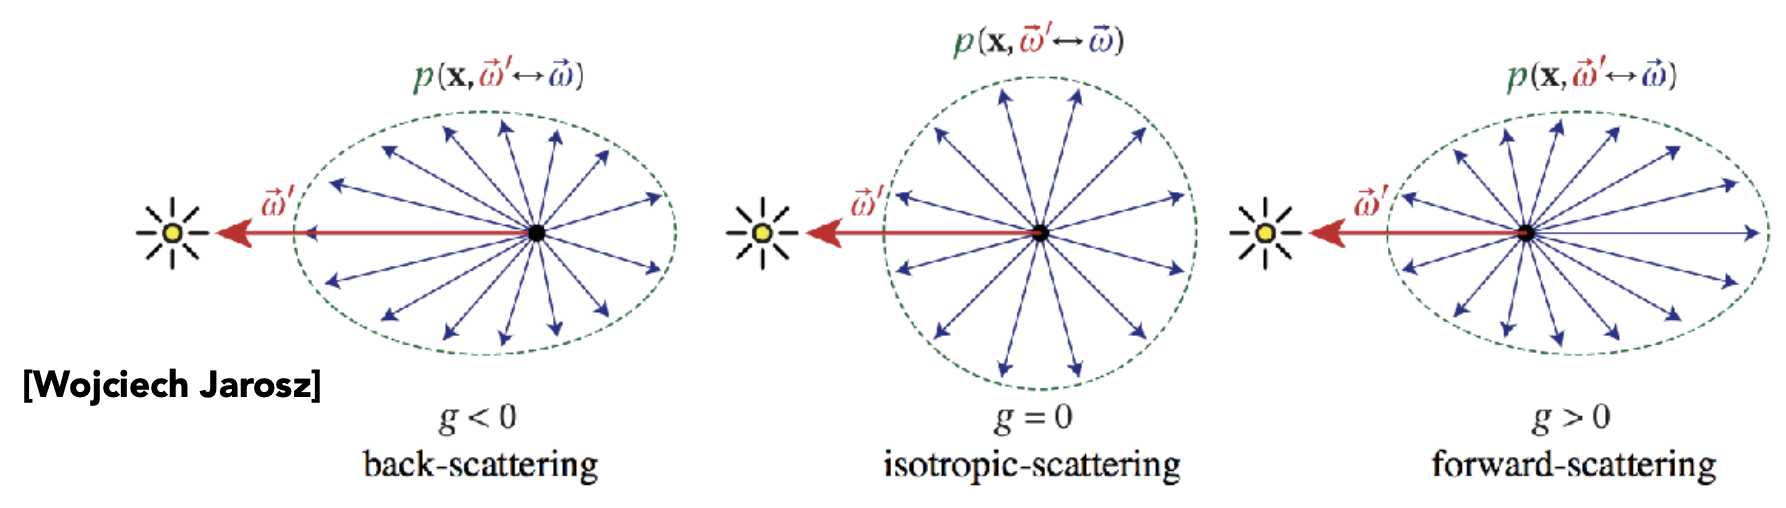
\includegraphics[scale=.35]{phasefunction.png}
	\caption{相位函数}
	\label{fig:pf}
\end{figure}

在渲染时我们会随机选择一个方向进行弹射, 随机选择一个方向直接进行传播, 在每一个点上和光线相连. 

\subsubsection{毛发}

光线和头发的作用不是简单的光线和表面的作用. 首先, 我们将头发看作一个圆柱体. 在Kajiya-Kay模型中, 我们认为一束光射到头发上后, 头发可以将光线散射成一个圆锥. 但是这种模型渲染出来的效果不好. 

\begin{figure}[H]
	\centering
	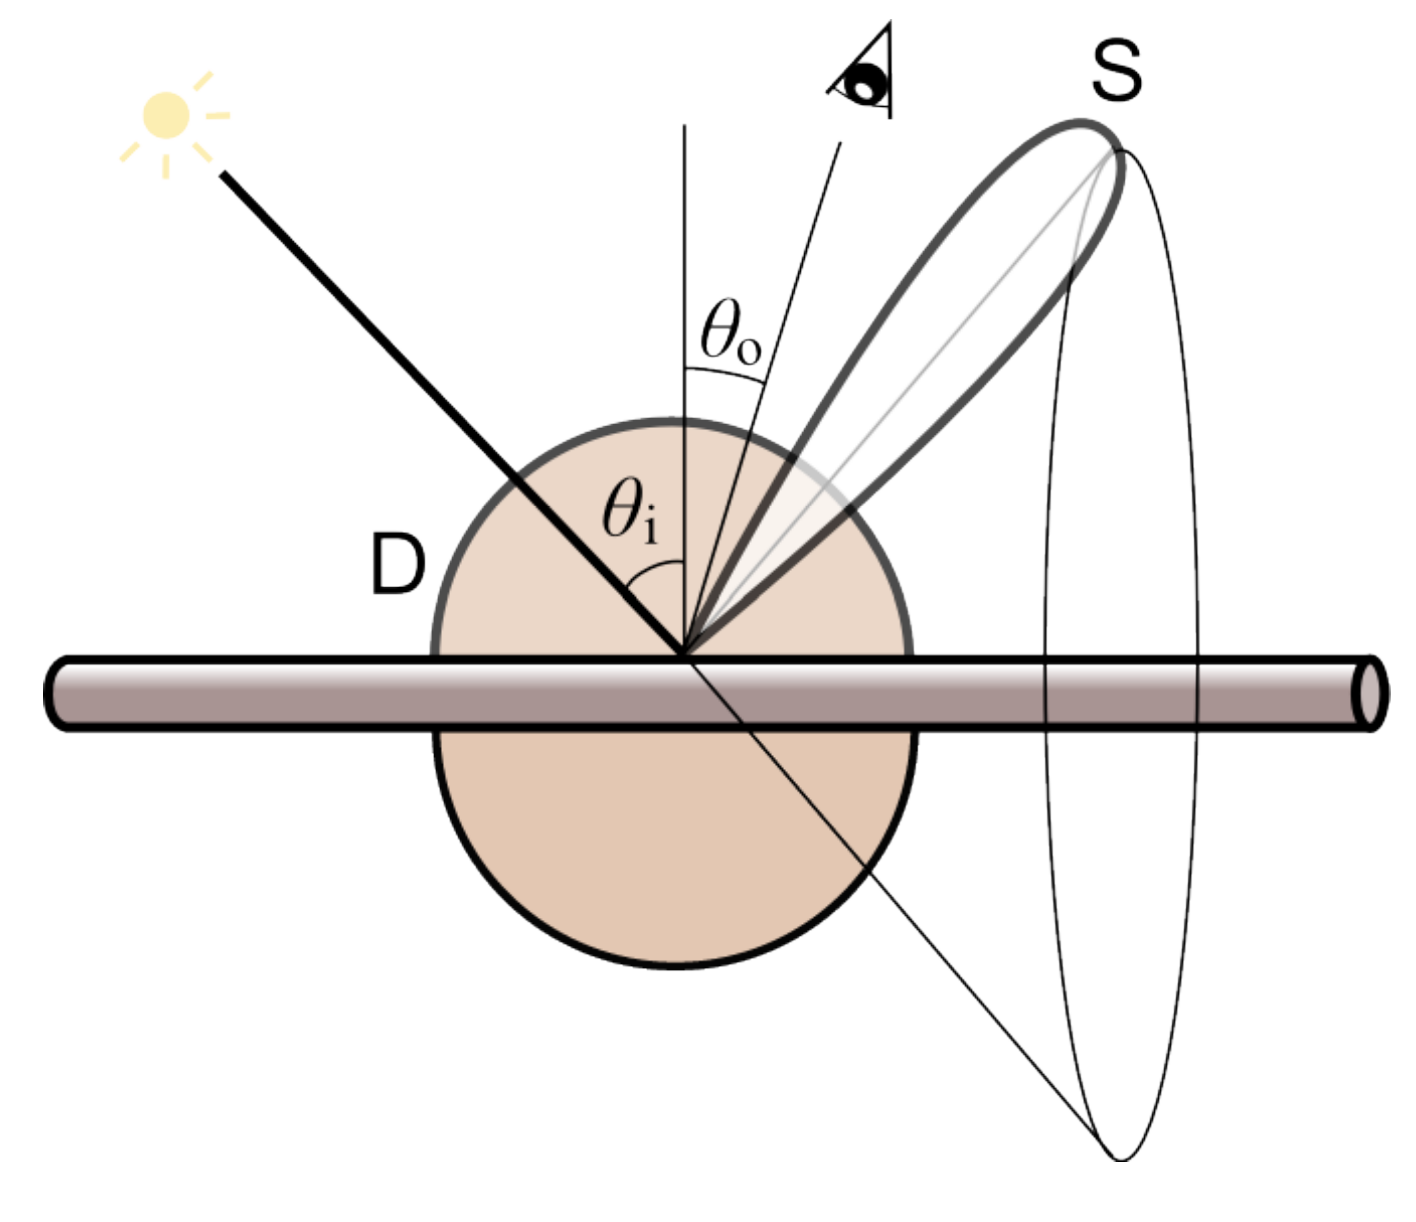
\includegraphics[scale=.15]{kkmodel.png}
	\caption{Kajiya-Kay模型}
	\label{fig:kk}
\end{figure}

Marschner模型认为, 头发是一个能够透光的``玻璃”, 因此光线应该分为三部分, 分别是: 
\begin{itemize}
	\item R: 光线直接反射光; 
	\item TT: 光线经过两次折射后射出的折射光; 
	\item TRT: 光线折射后经过一次介质内反射后的折射光. 
\end{itemize}

\begin{figure}[H]
	\centering
	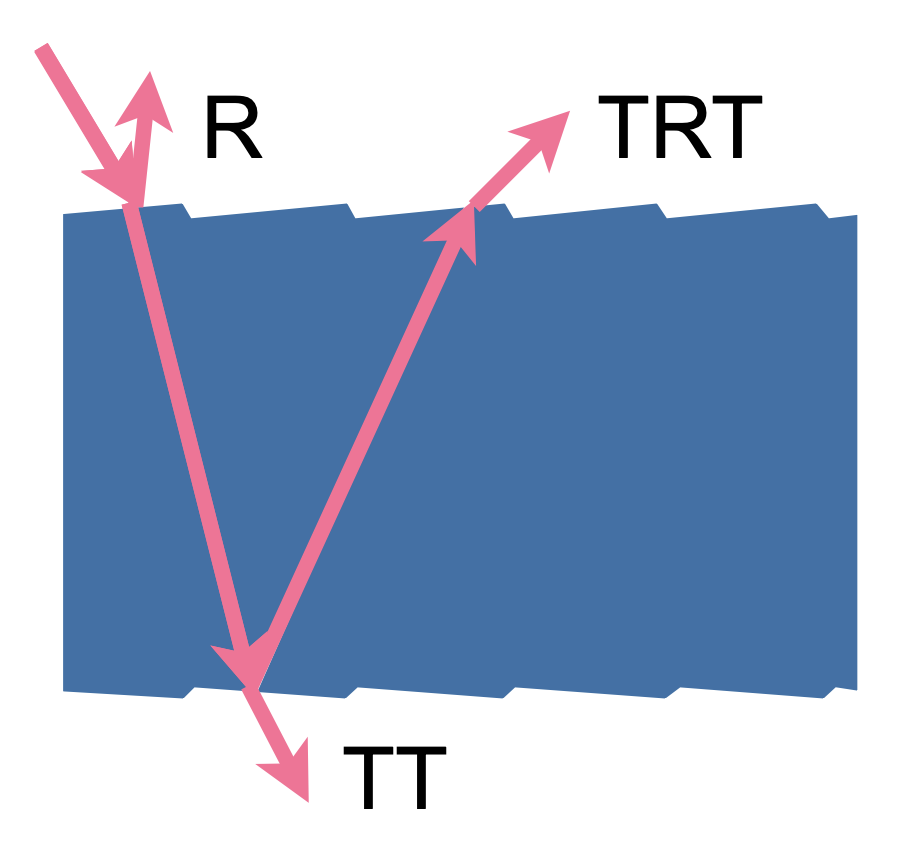
\includegraphics[scale=.25]{mmodel.png}
	\caption{Marschner模型}
	\label{fig:mm}
\end{figure}

以上的模型对于人类的毛发已经有了很好的表现, 但是对于动物毛发来说, 表现并不好. 这是因为动物的毛发并不是单层的结构. 动物毛发中包含一层毛髓质 (Medulla) , 因此引入双层模型 (Double Cylinder Model) 来对毛发进行建模. 

\begin{figure}[H]
	\centering
	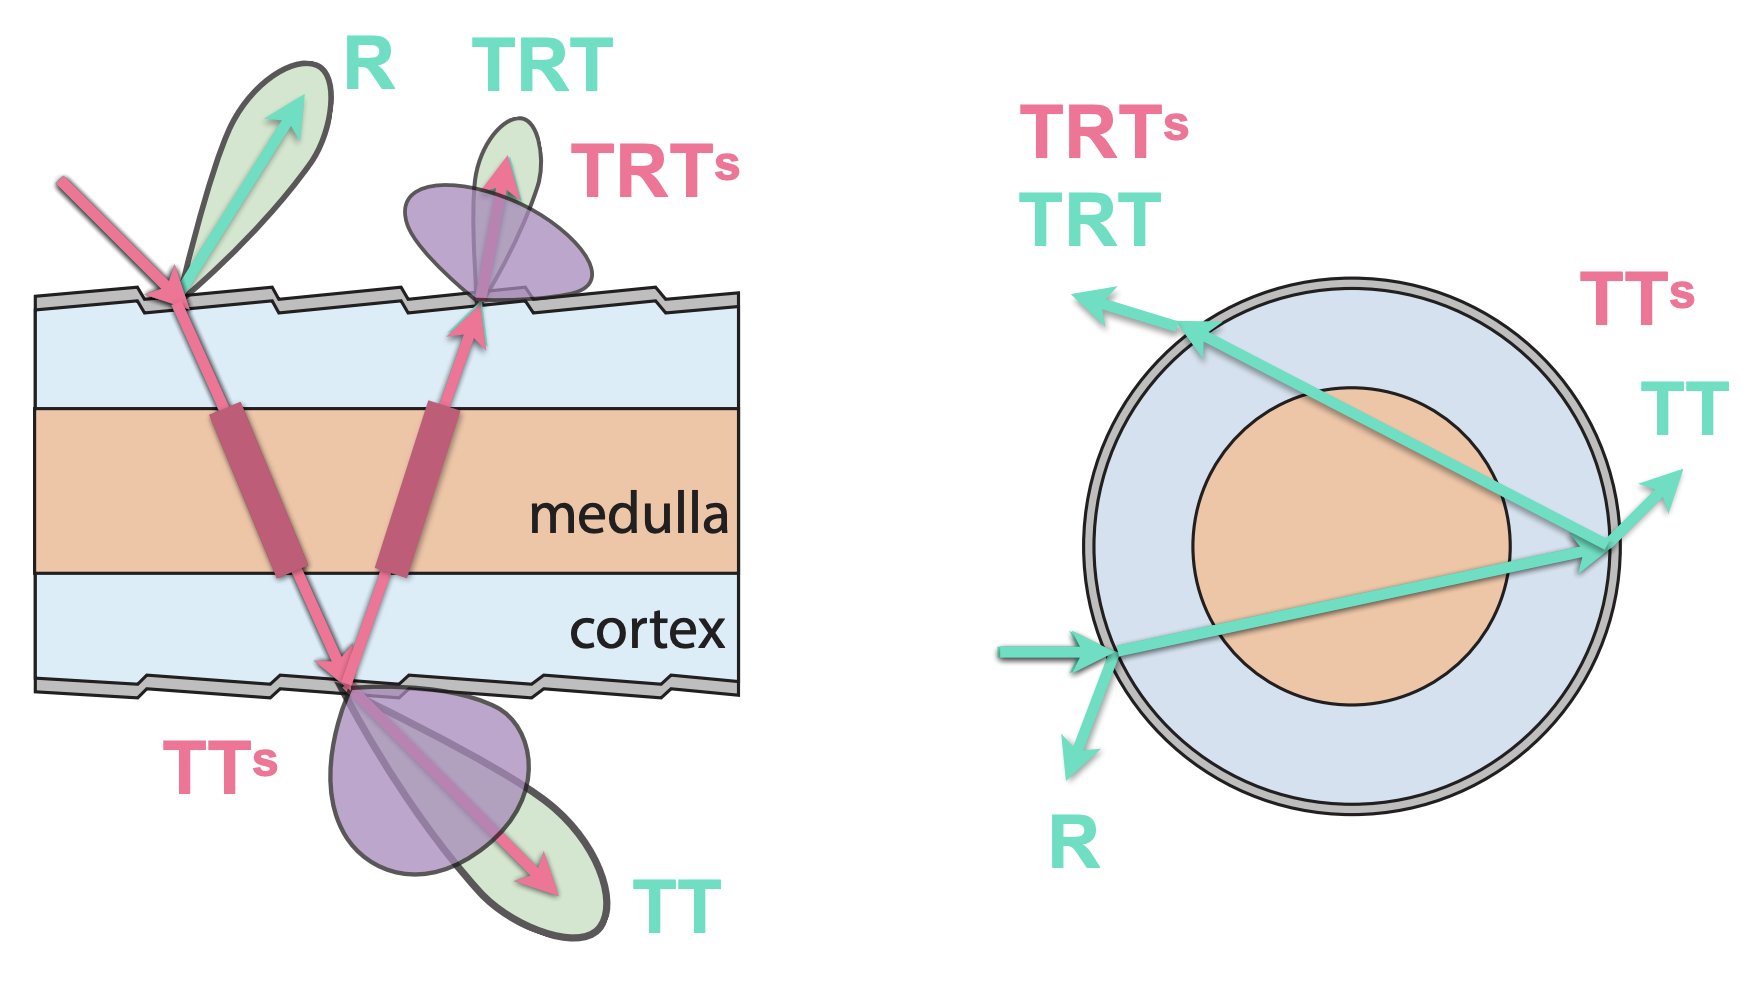
\includegraphics[scale=.25]{dcmodel.png}
	\caption{Double Cylinder模型}
	\label{fig:dc}
\end{figure}

在这个模型中我们额外增加了两种光: 
\begin{itemize}
	\item TT$^s$: 经过了中间介质的TT光线; 
	\item TRT$^s$: 经过了中间介质的TRT光线. 
\end{itemize}

这样5种光线结合在一起得到的毛发会更加的真实. 

\subsubsection{粒状材质}

\textbf{粒状材质 (Granular Material) }是由细小的颗粒组成的材质, 例如谷物, 沙子, 调味料等. 这样的材质也有程序性的方法进行渲染. 

\subsection{表面模型}

\subsubsection{半透明材质}

\textbf{半透明材质 (Translucent Material) }指的是能够透光的一些材质, 光线可以从一个地方进去并从另一个地方出去. 例如玉石, 水母都是典型的半透明材质. 

由于一条光在半透明材质上入射后, 出射光的起点并不一定在入射点上, 因此我们需要对BRDF进行拓展. 此时BDRF就变成了BSSDRF, 此时我们需要引入新的位置参数, 我们不仅要对角度进行积分, 还要在面积上进行积分: 
\begin{eqnarray}
	S(x_i,\omega_i,x_o,\omega_o)
\end{eqnarray}

\begin{eqnarray}
	L\left(x_{o}, \omega_{o}\right)=\int_{A} \int_{H^{2}} S\left(x_{i}, \omega_{i}, x_{o}, \omega_{o}\right) L_{i}\left(x_{i}, \omega_{i}\right) \cos \theta_{i} \mathrm{~d} \omega_{i} \mathrm{~d} A
\end{eqnarray}

我们会等效的认为, 一个半透明材质上有一束光摄入相当于在介质的外部和内部各有一个光源. 

\subsubsection{织物}

\textbf{织物 (Cloth) }的制作工艺比较的复杂. 首先, 多层 (Ply) 缠绕会变成一根纱 (Yarn) , 多根纱相互缠绕就会变成一根线 (Fiber) . 我们可以使用两种编织工艺, 一种是机织 (Woven) , 通过线之间的经纬交叉得到布料, 另一种方式是手打 (Knitted) 的方式, 类似于织毛衣的过程. 

不同的布料有不同的BDRF, 常见的渲染方法有: 
\begin{itemize}
	\item 把布料看作非表面材质, 将纤维划分为多个小方格进行渲染, 每个小方格单独判断散射性质; 
	\item 最暴力的做法是直接计算每一个纤维的结果. 
\end{itemize}

当然, 对于天鹅绒材质等布料, 使用BDRF并不合适. 

\subsection{真实世界模型}

我们认为现在的渲染器渲染出的画面并不真实, 主要原因是这些渲染器过于完美. 在实际生活中的物体一般表面都会带有划痕, 会让物体表面看起来更真实. 

我们可以用微表面模型的发现分布来解决这种情况. 我们只需要在微表面模型的分布上加一些噪声, 就可以产生带有划痕的效果. 但是, 在这样的法线分布下, 光线很难反射到光源处. 因此, 我们的解决方案是, 我们对于每一个像素, 对应一部分法线分布$p-NDF$, 使用这一部分的法线总体分布进行路径追踪. 

此外, 目前研究比较前沿的问题还有\textbf{波动光学 (Wave Optics) }的渲染. 

\section{程序化生成}

\textbf{程序化生成 (Procedural Appearance) }指的是我们可以不定义一个纹理, 而是直接定义一个噪声, 通过噪声计算纹理. 木纹, 陶瓷都可以定制对应的纹理进行程序化的生成. 
